\documentclass[ALICE,manyauthors]{cernphprep}

\usepackage[comma,square,numbers,sort&compress]{natbib}
\usepackage{hyperref}
\usepackage{lineno}
%\linenumbers

\usepackage{multirow}

\begin{document}%

%%%%%%%%%%%%%%%  Title page %%%%%%%%%%%%%%%%%%%%%%%%
\begin{titlepage}
%
\PHyear{2015}
\PHnumber{XXX}      % required, will be obtained from PH
\PHdate{Day Month}  % required, will be obtained from PH
%

%%% Put your own title + short title here:
\title{$\Lambda$K femtoscopy in Pb-Pb collisions at $\sqrt{s_{\mathrm{NN}}} = $ 2.76 TeV}
\ShortTitle{$\Lambda$K femtoscopy in Pb-Pb collisions}   % appears on right page headers

%%% Do not change the next lines
\Collaboration{ALICE Collaboration\thanks{See Appendix~\ref{app:collab} for the list of collaboration members}}
\ShortAuthor{ALICE Collaboration} % appears on left page headers, do not change

\begin{abstract}
We present our femtoscopy analysis of $\Lambda$K correlations in Pb-Pb collisions at $\sqrt{s_{\mathrm{NN}}}$ = 2.76 TeV from ALICE.  The femtoscopic correlations result from strong final-state interactions, and are fit with a parametrization based on a model by Lednicky and Lyuboshitz.  This allows us to both characterize the emission source and measure the scattering parameters for the particle pairs.  We observe a large difference in the $\Lambda$K$^{+}$ and $\Lambda$K$^{-}$ correlations in pairs with low relative momenta.  This might suggest an effect arising from different quark-antiquark interactions between the pairs ($\mathrm{s}\bar{\mathrm{s}}$ in $\Lambda$K$^{+}$ and $\mathrm{u}\bar{\mathrm{u}}$ in $\Lambda$K$^{-}$), or from different net strangeness for each system.
\end{abstract}
\end{titlepage}
\setcounter{page}{2}

\section{Introduction}
\label{sec:Introduction}
This is where the introduction goes.

\section{Data Analysis}
\label{sec:DataAnalysis}
This is where the data analysis section goes.

The analysis used ``pass 2" reconstructed Pb-Pb data from LHC11h (AOD145).
The runlist was selected from runs with global quality tag ``1" in the ALICE Run Condition Table.
Approximately 40 million combined central, semi-central, and minimum bias events were analyzed.
Runs from both positive (++) and negative (-{}-) magnetic field polarity settings were used.

Run list:  	
170593, 170572, 170388, 170387, 170315, 170313, 170312, 170311, 170309, 170308, 170306, 170270, 170269, 170268, 170230, 170228, 170207, 170204, 170203, 170193, 170163, 170159, 170155, 170091, 170089, 170088, 170085, 170084, 170083, 170081, 170040, 170027, 169965, 169923, 169859, 169858, 169855, 169846, 169838, 169837, 169835, 169591, 169590, 169588, 169587, 169586, 169557, 169555, 169554, 169553, 169550, 169515, 169512, 169506, 169504, 169498, 169475, 169420, 169419, 169418, 169417, 169415, 169411, 169238, 169167, 169160, 169156, 169148, 169145, 169144, 169138, 169099, 169094, 169091, 169045, 169044, 169040, 169035, 168992, 168988, 168826, 168777, 168514, 168512, 168511, 168467, 168464, 168460, 168458, 168362, 168361, 168342, 168341, 168325, 168322, 168311, 168310, 168115, 168108, 168107, 168105, 168076, 168069, 167988, 167987, 167985, 167920, 167915

Analysis was also performed on the LHC12a17a\_fix (AOD149) Monte Carlo HIJING events for certain checks.  THERMINATOR2 was also used for certain aspects, such as transform matrices described feed-down contributions.

The analysis was performed on the PWGCF analysis train using AliRoot v5-08-18-1 and AliPhysics vAN-20161027-1.

The main classes utilized include: AliFemtoVertexMultAnalysis, AliFemtoEventCutEstimators, AliFemtoESDTrackCutNSigmaFilter, AliFemtoV0TrackCutNSigmaFilter, AliFemtoXiTrackCut, AliFemtoV0PairCut, AliFemtoV0TrackPairCut, AliFemtoXiTrackPairCut, and AliFemtoAnalysisLambdaKaon.
All of these classes are contained in /AliPhysics/PWGCF/FEMTOSCOPY/AliFemto and .../AliFemtoUser.


%%%%%%%%%%%%%%%%%%%%%%%%% EVENT SELECTION %%%%%%%%%%%%%%%%%%%%%%%%%%%%%%%%%%%%%%%%%%%%%%%%%%%%%%%%%%%%%%%%%%%%%%%%%%%%%%%%%%%%%%%%%
The events used in this study were selected with the class AliFemtoEventCutEstimators according to the following criteria:

\begin{itemize}
 \itemsep0em
 \item Triggers
 \begin{itemize}
  \itemsep0em
  \item minimum bias (kMB)
  \item central (kCentral)
  \item semi-central (kSemiCentral)
 \end{itemize}
 \item z-position of reconstructed event vertex must be within 10 cm of the center of the ALICE detector
 \item the event must contain at least one particle of each type from the pair of interest
\end{itemize}

The event mixing was handled by the AliFemtoVertexMultAnalysis class, which only mixes events with like vertex position and centrality.
The following criteria were used for event mixing:

\begin{itemize}
 \itemsep0em
 \item Number of events to mix = 5
 \item Vertex position bin width = 2 cm
 \item Centrality bin width = 5%
\end{itemize}

The AliFemtoEventReaderAODChain class is used to read the events.
Event flatteneing is not currently used.
FilterBit(7).
The centrality is determined by the ``V0M" method of AliCentrality, set by calling AliFemtoEventReaderAOD::SetUseMultiplicity(kCentrality).
I utilize the SetPrimaryVertexCorrectionTPCPoints switch, which causes the reader to shift all TPC points to be relative to the event vertex.







\subsection{V0 selection}
\label{sec:V0Selection}
This is how we select V0s.

$\Lambda$ ($\bar{\Lambda}$) and K$^{0}_{S}$ are neutral particles which cannot be directly detected, but must instead be reconstructed through detection of their decay products, or daughters.  
This process is illustrated in Figure \ref{fig:V0Reconstruction}.
In general, particles which are topologically reconstructed in this fashion are called V0 particles.
The class AliFemtoV0TrackCutNSigmaFilter (which is an extension of AliFemtoV0TrackCut) is used to reconstruct the V0s.

In order to obtain a true and reliable signal, one must ensure good purity of the V0 collection.  The purity of the collection is calculated as:

\begin{equation}
 Purity = \frac{Signal}{Signal + Background}
\label{eqn:Purity}
\end{equation}

To obtain both the signal and background, the invariant mass distribution (m$_{inv}$) of all V0 candidates must be constructed immediately before the final invariant mass cut.
Examples of such distribtions can be found in Figures \ref{fig:cLamPurity} and \ref{fig:K0Purity}.
It is vital that this distribution be constructed immediately before the final m$_{inv}$ cut, otherwise it would be impossible to estimate the background.
As shown in Figures \ref{fig:cLamPurity} and \ref{fig:K0Purity}, the background is fit (with a polynomial) outside of the peak region of interest to obtain an estimate for the backfround within the region.
Within the m$_{inv}$ cut limits, the background is the region below the fit while the signal is the region above the fit.

\begin{figure}[h]
  \centering
  \includegraphics[width=0.5\textwidth]{/home/jesse/Analysis/FemtoAnalysis/LamKPublication/Figures/PDF/V0CutsGeneral.pdf}
  \caption[V0 Reconstruction]{V0 Reconstruction}
  \label{fig:V0Reconstruction}
\end{figure}


\subsubsection{$\Lambda$ selection}
\label{sec:LambdaSelection}
The following cuts were used to select good $\Lambda$ ($\bar{\Lambda}$) candidates: 


\begin{table}[htbp]
 \centering
%  \renewcommand{\arraystretch}{1.5}
  \begin{tabular}{lc|c|l}
   \hline  
   \multicolumn{4}{c}{$\Lambda$ selection} \\
   \hline
   \multicolumn{3}{l|}{$|\eta|$} & $< 0.8$ \\
   \hline
   \multicolumn{3}{l|}{$p_{\mathrm{T}}$} & $> 0.4$ GeV/\textit{c} \\
   \hline
   \multicolumn{3}{l|}{$|m_{\mathrm{inv}} - m_{\mathrm{PDG}}|$} & $< 3.8$ MeV \\ 
   \hline
   \multicolumn{3}{l|}{DCA to prim. vertex} & $<$ 0.5 cm \\
   \hline
   \multicolumn{3}{l|}{Cosine of pointing angle} & $>$ 0.9993 \\
   \hline
   \multicolumn{3}{l|}{OnFlyStatus} & false \\
   \hline
   \multicolumn{3}{l|}{Decay Length} & $<$ 60 cm \\
   \hline
   \multicolumn{3}{l|}{Shared Daughter Cut} & true \\
   \hline
   \multicolumn{3}{l|}{Misidentification Cut} & true \\
   \hline   
   
   
   \multicolumn{4}{c}{Daughter Cuts ($\pi$ and p)} \\
   \hline
   \multicolumn{3}{l|}{$|\eta|$} &  $< 0.8$ \\
   \hline
   \multicolumn{3}{l|}{SetTPCnclsDaughters} & (80) \\
   \hline
   \multicolumn{3}{l|}{SetStatusDaughters} & (AliESDtrack::kTPCrefit) \\
   \hline
   \multicolumn{3}{l|}{DCA $\pi$p Daughters} & $<$ 0.4 cm \\
   \hline
   
   
   \multicolumn{4}{c}{$\pi$-specific cuts} \\
   \hline
   \multicolumn{3}{l|}{$p_{\mathrm{T}}$} & $> 0.16$ GeV/\textit{c} \\
   \hline
   \multicolumn{3}{l|}{DCA to prim vertex} & $>$ 0.3 cm \\
   \hline
   \multicolumn{4}{l}{TPC and TOF N$\sigma$ Cuts} \\
   \hline
    & \multicolumn{1}{c}{$p <$ 0.5 GeV/\textit{c}} &  & N$\sigma_{\mathrm{TPC}} <$ 3 \\
   \hline
    & \multirow{2}{*}{$p >$ 0.5 GeV/\textit{c}} &  if TOF \& TPC available & N$\sigma_{\mathrm{TPC}} <$ 3 \& N$\sigma_{\mathrm{TOF}} <$ 3 \\
   \cline{3-4}
    & & else & N$\sigma_{\mathrm{TOF}} <$ 3 \\
   \hline
   
   
   \multicolumn{4}{c}{p-specific cuts} \\
   \hline
   \multicolumn{3}{l|}{$p_{\mathrm{T}}$} & $ > $ 0.5($p$) [0.3($\bar{p}$)] GeV/\textit{c} \\
   \hline
   \multicolumn{3}{l|}{DCA to prim vertex} & $>$ 0.1 cm \\
   \hline
   \multicolumn{4}{l}{TPC and TOF N$\sigma$ Cuts} \\
   \hline
    & \multicolumn{1}{c}{$p <$ 0.8 GeV/\textit{c}} & & N$\sigma_{\mathrm{TPC}} <$ 3 \\
   \hline
    & \multirow{2}{*}{$p >$ 0.8 GeV/\textit{c}} &  if TOF \& TPC available & N$\sigma_{\mathrm{TPC}} <$ 3 \& N$\sigma_{\mathrm{TOF}} <$ 3 \\
   \cline{3-4}
    & & else & N$\sigma_{\mathrm{TOF}} <$ 3 \\
   \hline   
  \end{tabular}
% \end{minipage}
 \caption{$\Lambda$ selection}
 \label{tab:LamCuts} 
\end{table}


Shared daughter cut iterates through V0 collection to ensure that no daughter is used in more than one V0 candidate

Figure \ref{fig:MassAssK0ShortHyp_cLamK0:a} shows the mass assuming K$^{0}_{S}$ hypothesis for the $\Lambda$ collection, i.e. assume the daughters are $\pi^{+}\pi^{-}$ instead of $\pi^{+}\bar{p}^{-}$.
Figure \ref{fig:MassAssK0ShortHyp_cLamK0:b} is a similar plot, but is for the $\bar{\Lambda}$ collection, i.e. assume the daughters are $\pi^{+}\pi^{-}$ instead of $\pi^{+}\bar{p}^{-}$.
The K$^{0}_{S}$ contamination is visible, although not profound, in both in the slight peaks around $m_{\mathrm{inv}}$ = 0.497 GeV/$c^{2}$.
If one simply cuts out the entire peak, good $\Lambda$ particles will be lost.
Ideally, the $\Lambda$ selection and K$^{0}_{S}$ misidentification cuts are selected such that the peak is removed from this plot while leaving the distribution continuous.
To attempt to remove these K$^{0}_{S}$ contaminations without throwing away good $\Lambda$ and $\bar{\Lambda}$ particles, the following misidentification cuts are imposed; a $\Lambda$($\bar{\Lambda}$) candidate is rejected if all of the following criteria are satisfied:
\begin{itemize}
 \item $\left|m_{\mathrm{inv,~ K^{0}_{S}~ Hypothesis}} - m_{\mathrm{PDG,~ K^{0}_{S}}}\right| < $ 9.0 MeV/c$^{2}$
 \item Positive and negative daughters pass $\pi$ daughter cut implemented for K$^{0}_{S}$ reconstruction
 \item $\left|m_{\mathrm{inv,~ K^{0}_{S}~ Hypothesis}} - m_{\mathrm{PDG,~ K^{0}_{S}}}\right|~ < ~\left|m_{\mathrm{inv,~ \Lambda(\bar{\Lambda})~ Hypothesis}} - m_{\mathrm{PDG,~ \Lambda(\bar{\Lambda})}}\right|$
\end{itemize} 


Figure \ref{fig:cLamPurity} shows the invariant mass (m$_{\mathrm{inv}}$) distribution of all $\Lambda$($\bar{\Lambda}$) candidates immediately before the final invariant mass cut.
These distributions are used to calculate the collection purities.
The $\Lambda$ and $\bar{\Lambda}$ purities are found to be: Purity($\Lambda$) $\approx$ Purity($\bar{\Lambda}$) $\approx$ 95\%.


\begin{figure}[b]
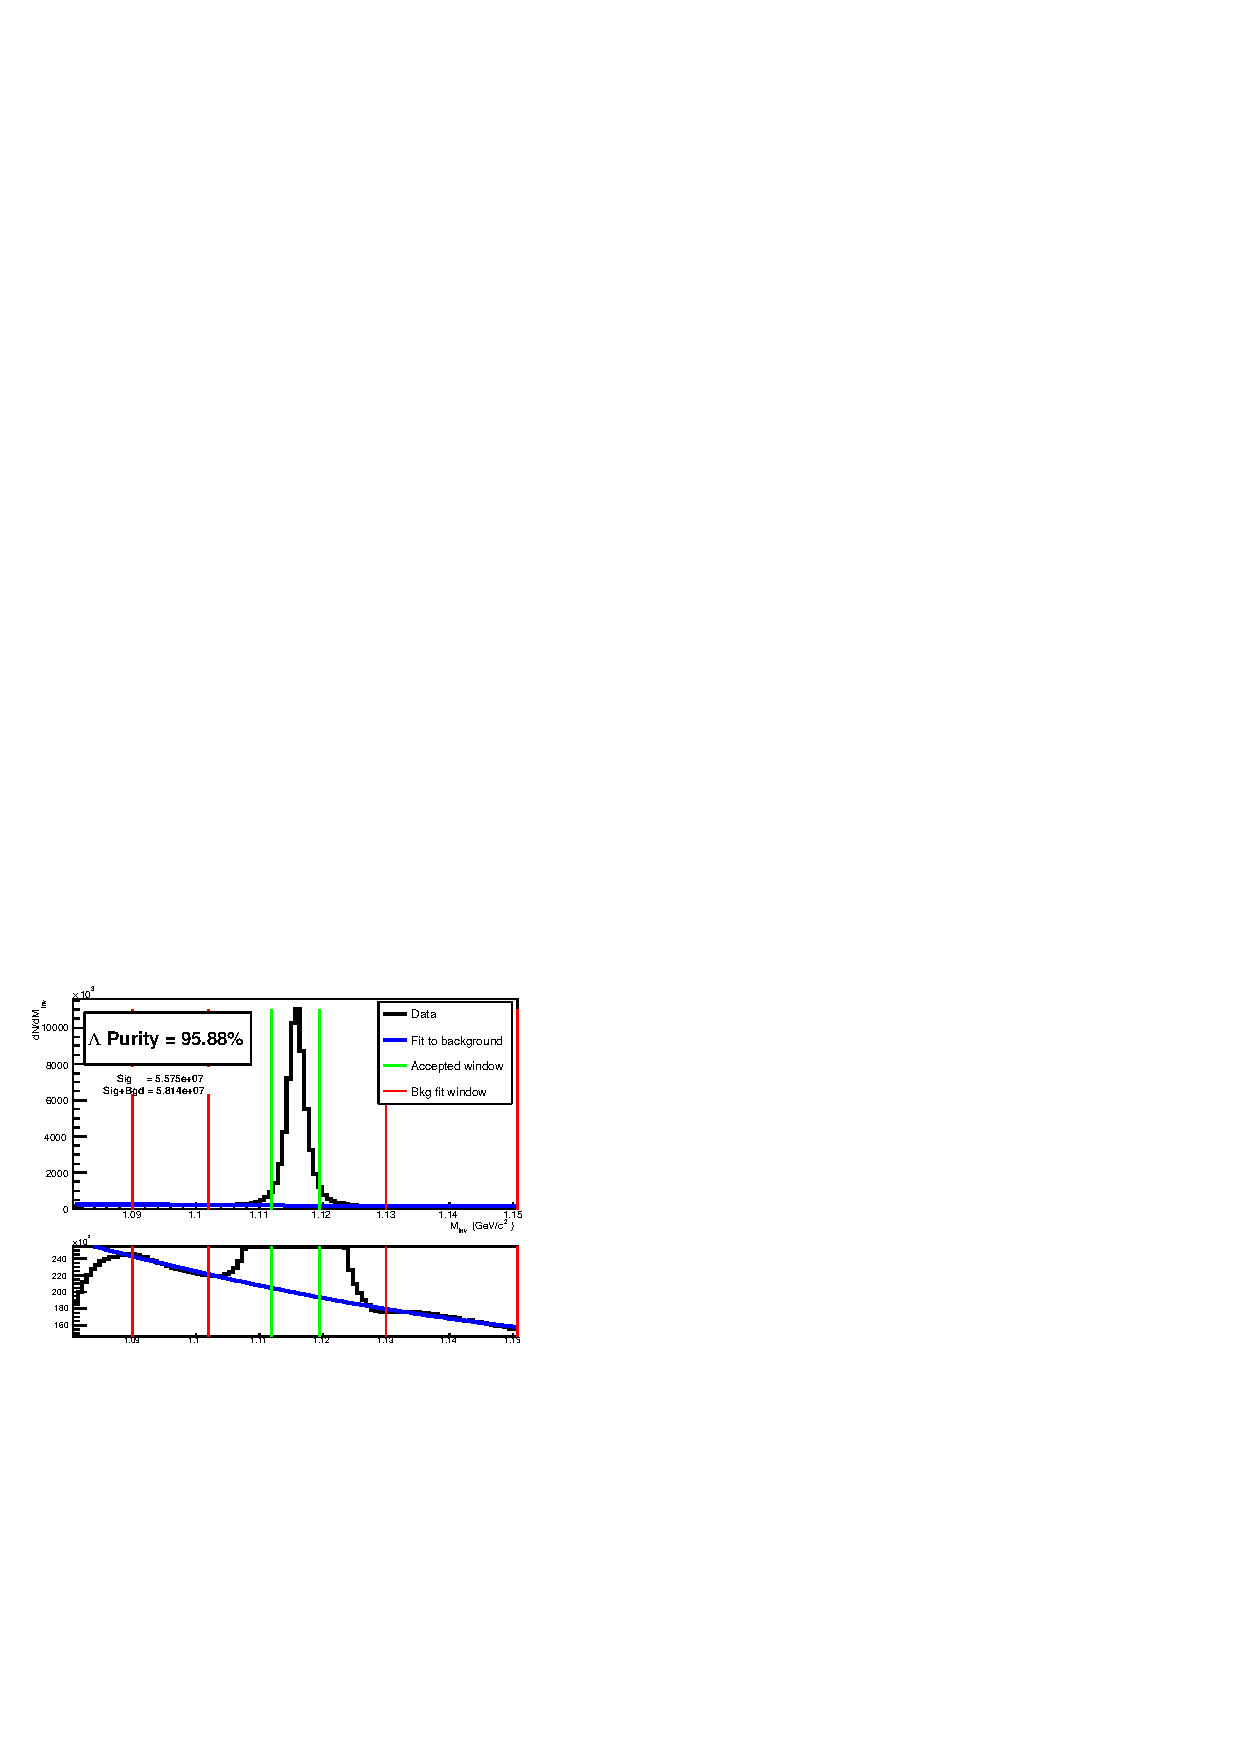
\includegraphics{/home/jesse/Analysis/FemtoAnalysis/LamKPublication/Figures/PDF/LamPurity_LamK0.pdf}% Here is how to import EPS art
\caption{\label{fig:epsart} A figure caption. The figure captions are
automatically numbered.}
\end{figure}

\subsubsection{K$^{0}_{S}$ selection}
\label{sec:K0sSelection}
The following cuts were used to select good K$^{0}_{S}$ candidates:



\begin{table}[htbp]
 \centering
%  \renewcommand{\arraystretch}{1.5}
  \begin{tabular}{lc|c|l}
   \hline  
   \multicolumn{4}{c}{K$^{0}_{S}$ selection} \\
   \hline
   \multicolumn{3}{l|}{$|\eta|$} & $< 0.8$ \\
   \hline
   \multicolumn{3}{l|}{$p_{\mathrm{T}}$} & $> 0.2$ GeV/\textit{c} \\
   \hline
   \multicolumn{4}{l|}{$m_{PDG}-13.677 \ \mathrm{MeV} < m_{\mathrm{inv}} < m_{\mathrm{PDG}} + 2.0323 \ \mathrm{MeV}$} \\ 
   \hline
   \multicolumn{3}{l|}{DCA to prim. vertex} & $<$ 0.3 cm \\
   \hline
   \multicolumn{3}{l|}{Cosine of pointing angle} & $>$ 0.9993 \\
   \hline
   \multicolumn{3}{l|}{OnFlyStatus} & false \\
   \hline
   \multicolumn{3}{l|}{Decay Length} & $<$ 30 cm \\
   \hline
   \multicolumn{3}{l|}{Shared Daughter Cut} & true \\
   \hline
   \multicolumn{3}{l|}{Misidentification Cut} & true \\
   \hline   
      
   
   \multicolumn{4}{c}{$\pi^{\pm}$ Daughter Cuts} \\
   \hline
   \multicolumn{3}{l|}{$|\eta|$} &  $< 0.8$ \\
   \hline
   \multicolumn{3}{l|}{SetTPCnclsDaughters} & (80) \\
   \hline
   \multicolumn{3}{l|}{SetStatusDaughters} & (AliESDtrack::kTPCrefit) \\
   \hline
   \multicolumn{3}{l|}{DCA $\pi^{+}\pi^{-}$ Daughters} & $<$ 0.3 cm \\
   \hline
   \multicolumn{3}{l|}{$p_{\mathrm{T}}$} & $>$ 0.15 GeV/\textit{c} \\
   \hline
   \multicolumn{3}{l|}{DCA to prim vertex} & $>$ 0.3 cm \\
   \hline
   \multicolumn{4}{l}{TPC and TOF N$\sigma$ Cuts} \\
   \hline
    & \multicolumn{1}{c}{$p <$ 0.5 GeV/\textit{c}} &  & N$\sigma_{\mathrm{TPC}} <$ 3 \\
   \hline
    & \multirow{2}{*}{$p >$ 0.5 GeV/\textit{c}} &  if TOF \& TPC available & N$\sigma_{\mathrm{TPC}} <$ 3 \& N$\sigma_{\mathrm{TOF}} <$ 3 \\
   \cline{3-4}
    & & else & N$\sigma_{\mathrm{TOF}} <$ 3 \\
   \hline   
  \end{tabular}
% \end{minipage}
 \caption{K$^{0}_{S}$ selection}
 \label{tab:K0sCuts} 
\end{table}

As can be seen in Figure \ref{fig:MassAsscLamHyp}, some misidentified $\Lambda$ and $\bar{\Lambda}$ particles contaminate our K$^{0}_{S}$ sample.
Figure \ref{fig:MassAsscLamHyp:a} shows the mass assuming $\Lambda$-hypothesis for the K$^{0}_{S}$ collection, i.e. assume the daughters are $p^{+}\pi^{-}$ instead of $\pi^{+}\pi^{-}$.
Figure \ref{fig:MassAsscLamHyp:b} is similar, but shows the mass assuming $\bar{\Lambda}$ hypothesis for the collection, i.e. assume the daughters are $\pi^{+}\bar{p}^{-}$ instead of $\pi^{+}\pi^{-}$.
The $\Lambda$ contamination can be seen in \ref{fig:MassAsscLamHyp:a}, and the $\bar{\Lambda}$ contamination in \ref{fig:MassAsscLamHyp:b}, in the peaks around $m_{\mathrm{inv}}$ = 1.115 GeV/$c^{2}$.
Additionally, the $\bar{\Lambda}$ contamination is visible in Figure \ref{fig:MassAsscLamHyp:a}, and the $\Lambda$ contamination visible in Figure \ref{fig:MassAsscLamHyp:b}, in the region of excess around 1.65 $<$ $m_{\mathrm{inv}}$ $<$ 2.1 GeV/$c^{2}$.
This is confirmed as the number of misidentified $\Lambda$ particles in the sharp peak of Figure \ref{fig:MassAsscLamHyp:a} (misidentified $\bar{\Lambda}$ particles in the sharp peak of Figure \ref{fig:MassAsscLamHyp:b}) approximately equals the excess found in the 1.65 $<$ $m_{\mathrm{inv}}$ $<$ 2.1 GeV/$c^{2}$ region of Figure \ref{fig:MassAsscLamHyp:a} (Figure \ref{fig:MassAsscLamHyp:b}).

The peaks around $m_{\mathrm{inv}} = $ 1.115 GeV/$c^{2}$ in Figure \ref{fig:MassAsscLamHyp} contain both misidentified $\Lambda$ ($\bar{\Lambda}$) particles and good K$^{0}_{S}$.
If one simply cuts out the entire peak, some good K$^{0}_{S}$ particles will be lost.
Ideally, the K$^{0}_{S}$ selection and $\Lambda$($\bar{\Lambda}$) misidentification cuts can be selected such that the peak is removed from this plot while leaving the distribution continuous.
To attempt to remove these $\Lambda$ and $\bar{\Lambda}$ contaminations without throwing away good K$^{0}_{S}$ particles, the following misidentification cuts are imposed; a K$^{0}_{S}$ candidate is rejected if all of the following criteria are satisfied (for either $\Lambda$ or $\bar{\Lambda}$ hypothesis):
\begin{itemize}
 \item $\left|m_{\mathrm{inv}, \ \Lambda(\bar{\Lambda}) \ \mathrm{Hypothesis}} - m_{\mathrm{PDG},\ \Lambda(\bar{\Lambda})}\right| < $ 9.0 MeV/$c^{2}$
 \item Positive daughter passes $p^{+}$($\pi^{+}$) daughter cut implemented for $\Lambda$($\bar{\Lambda}$) reconstruction
 \item Negative daughter passes $\pi^{-}$($\bar{p}^{-}$) daughter cut implemented by $\Lambda$($\bar{\Lambda}$) reconstruction
 \item $\left|m_{\mathrm{inv}, \ \Lambda(\bar{\Lambda}) \ \mathrm{Hypothesis}} - m_{\mathrm{PDG},\ \Lambda(\bar{\Lambda})}\right|~ < ~\left|m_{\mathrm{inv},~ \mathrm{K}^{0}_{S}~ \mathrm{Hypothesis}} - m_{\mathrm{PDG},~ \mathrm{K}^{0}_{S}}\right|$
\end{itemize} 


\begin{figure*}
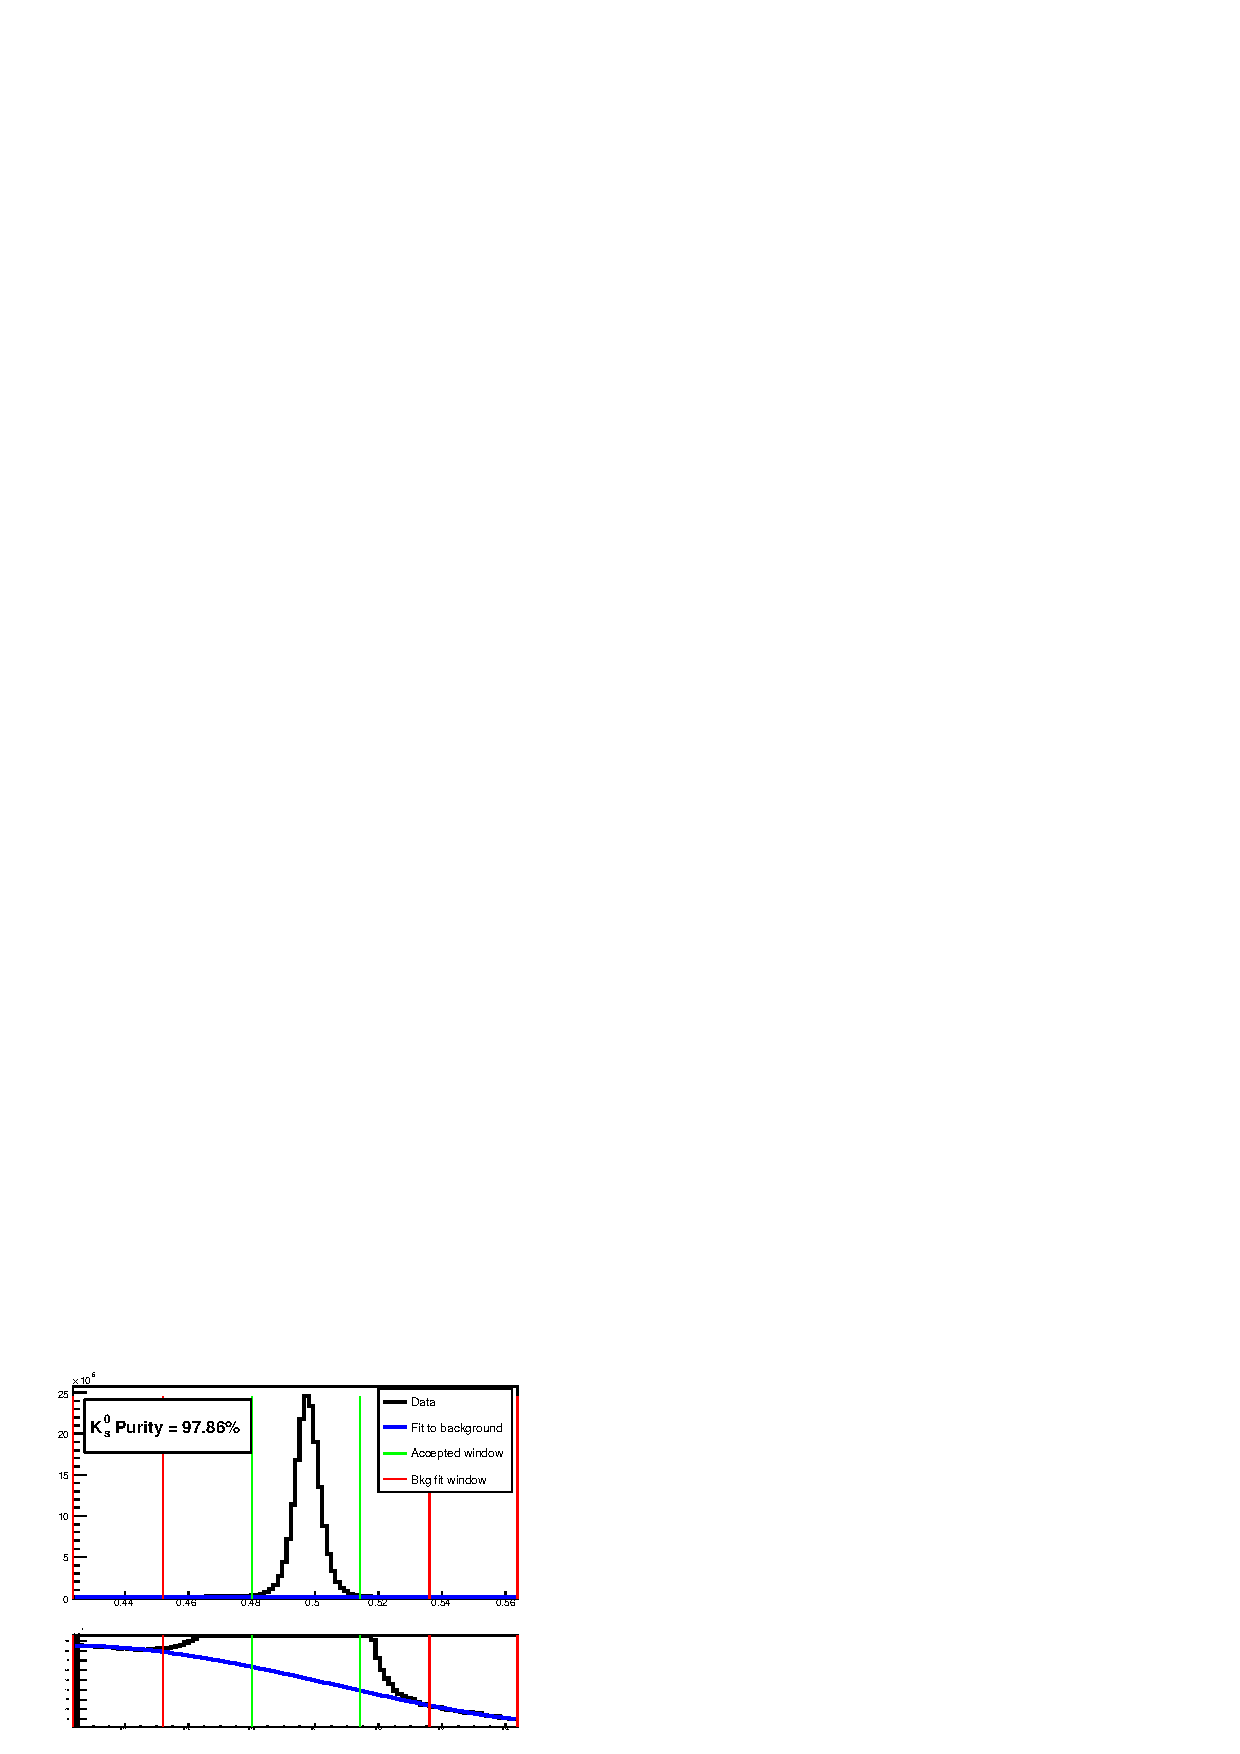
\includegraphics{/home/jesse/Analysis/FemtoAnalysis/LamKPublication/Figures/PDF/K0Purity_LamK0.pdf}% Here is how to import EPS art
\caption{\label{fig:wide}Use the figure* environment to get a wide
figure that spans the page in \texttt{twocolumn} formatting.}
\end{figure*}

\subsection{K$^{\pm}$ selection}
\label{sec:KchSelection}
This is how we select K$^{\mathrm{ch}}$ or K$^{\pm}$ candidates.

\begin{figure}[b]
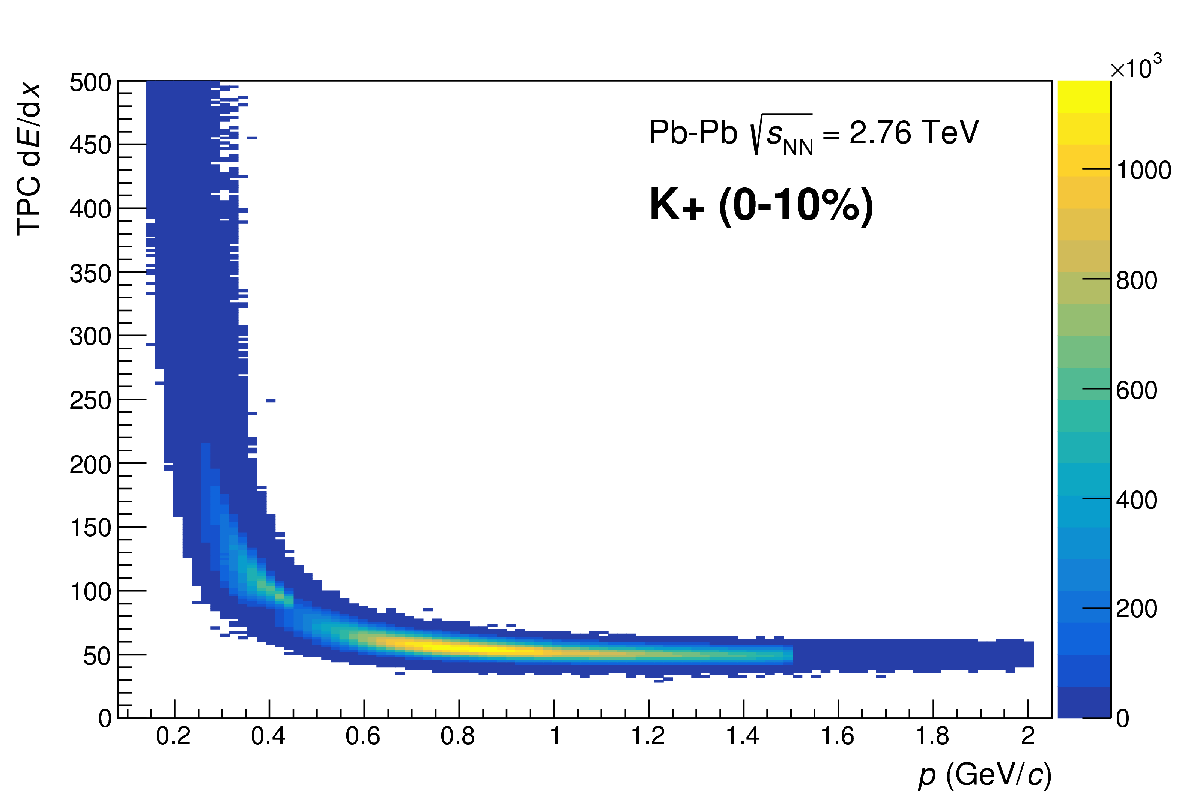
\includegraphics[width=1.0\textwidth]{/home/jesse/Analysis/FemtoAnalysis/LamKPublication/Figures/PDF/canDrawKchdEdx_LamKchP_0010_KchP.pdf}% Here is how to import EPS art
\caption{\label{fig:epsart} A figure caption. The figure captions are
automatically numbered.}
\end{figure}

Charged kaons are identified using the AliFemtoESDTrackCutNSigmaFilter class.  The specific cuts used in this analysis are as follows:

\begin{table}[htbp]
 \centering
%  \renewcommand{\arraystretch}{1.5}
  \begin{tabular}{lc|c|l}
   \hline  
   \multicolumn{4}{c}{K$^{\pm}$ selection} \\
   \hline
   \multicolumn{3}{l|}{$|\eta|$} & $< 0.8$ \\
   \hline
   \multicolumn{3}{l|}{$p_{\mathrm{T}}$} & 0.14 $< p_{\mathrm{T}} < 1.5$ GeV/\textit{c} \\
   \hline
   \multicolumn{3}{l|}{FilterBit} & 7 \\
   \hline
   \multicolumn{3}{l|}{Min. number of clusters in the TPC} & 80 \\
   \hline
   \multicolumn{3}{l|}{Max. allowed $\chi^{2}/N_{DOF}$ for ITS clusters} & 3.0 \\
   \hline
   \multicolumn{3}{l|}{Max. allowed $\chi^{2}/N_{DOF}$ for TPC clusters} & 4.0 \\
   \hline   
   \multicolumn{3}{l|}{Maximum XY impact parameter} & 2.4 cm \\
   \hline
   \multicolumn{3}{l|}{Maximum Z impact parameter} & 3.0 cm \\
   \hline
   \multicolumn{3}{l|}{Remove particles with any kink labels} & true \\
   \hline
   \multicolumn{3}{l|}{Maximum allowed sigma to primary vertex} & 3.0 \\
   \hline   
   
   \multicolumn{4}{l}{PID Probabilities} \\
   \hline
    & \multicolumn{2}{l|}{K} & $>$ 0.2 \\
   \hline
    & \multicolumn{2}{l|}{$\pi$} & $<$ 0.1 \\
   \hline
    & \multicolumn{2}{l|}{$\mu$} & $<$ 0.8 \\
   \hline
    & \multicolumn{2}{l|}{p} & $<$ 0.1 \\
   \hline
   
   \multicolumn{3}{l|}{Most probable particle type} & Kaon (fMostProbable=3) \\
   \hline
   
   \multicolumn{4}{l}{TPC and TOF N$\sigma$ Cuts} \\
   \cline{2-4}
    & \multicolumn{1}{l}{$p <$ 0.4 GeV/\textit{c}} &  & N$_{\sigma \mathrm{K,TPC}} <$ 2 \\
   \cline{2-4}
    & \multicolumn{1}{l}{0.4 $< p <$ 0.45 GeV/\textit{c}} & & N$_{\sigma \mathrm{K,TPC}} <$ 1 \\
   \cline{2-4}     
    & \multicolumn{1}{l}{0.45 $< p <$ 0.80 GeV/\textit{c}} & & N$_{\sigma \mathrm{K,TPC}} <$ 3 \& N$_{\sigma \mathrm{K,TOF}} <$ 2 \\ 
   \cline{2-4}
    & \multicolumn{1}{l}{0.80 $< p <$ 1.0 GeV/\textit{c}} & & N$_{\sigma \mathrm{K,TPC}} <$ 3 \& N$_{\sigma \mathrm{K,TOF}} <$ 1.5 \\ 
   \cline{2-4}
    & \multicolumn{1}{l}{$p >$ 1.0 GeV/\textit{c}} & & N$_{\sigma \mathrm{K,TPC}} <$ 3 \& N$_{\sigma \mathrm{K,TOF}} <$ 1 \\ 
   \hline
   \multicolumn{3}{l|}{Electron Rejection} & Reject if N$_{\sigma e^{-},\mathrm{TPC}} < $ 3 \\
   \hline
   
   \multicolumn{4}{l}{Pion Rejection:  Reject if:} \\
   \hline
   \multirow{3}{*}{$p <$ 0.65 GeV/\textit{c}} & if TOF and TPC available & \multicolumn{1}{c}{} & N$_{\sigma \pi,\mathrm{TPC}} <$ 3 \& N$_{\sigma \pi,\mathrm{TOF}} <$ 3 \\
   \cline{2-4}
    & \multirow{2}{*}{else} & $p <$ 0.5 GeV/\textit{c} & N$_{\sigma \pi,\mathrm{TPC}} <$ 3 \\
   \cline{3-4}
    &  & 0.5 $< p <$ 0.65 GeV/\textit{c} & N$_{\sigma \pi,\mathrm{TPC}} <$ 2 \\
   \cline{2-4}
   \multicolumn{3}{l|}{0.65 $< p <$ 1.5 GeV/\textit{c}} & N$_{\sigma \pi,\mathrm{TPC}} <$ 5 \& N$_{\sigma \pi,\mathrm{TOF}} <$ 3 \\
   \cline{2-4}
   \multicolumn{3}{l|}{$p >$ 1.5 GeV/\textit{c}} & N$_{\sigma \pi,\mathrm{TPC}} <$ 5 \& N$_{\sigma \pi,\mathrm{TOF}} <$ 2 \\
   \hline
  \end{tabular}
% \end{minipage}
 \caption{K$^{\pm}$ selection}
 \label{tab:KchCuts} 
\end{table}

The purity of the K$^{\pm}$ collections was estimated using the MC data, for which the true identity of each reconstructed K$^{\pm}$ particle is known.  Therefore, the purity may be estimated as:

\begin{equation}
 Purity(K^{\pm}) = \frac{N_{true}}{N_{reconstructed}} \\
\label{eqn:KchPurity}
\end{equation}

Purity(K$^{+}$) $\approx$ Purity(K$^{-}$) $\approx$ 97\%


\subsection{Pair Selection}
\label{PairSelection}

It is important to obtain true particle pairs in the analysis.  In particular, contamination from pairs constructed with split or merged tracks, and pairs sharing daughters, can introduce an artificial signal into the correlation function, obscuring the actual physics.

\begin{enumerate}
 \item Shared Daughter Cut for Pairs
 \begin{enumerate}
  \item V0-V0 Pairs (i.e. $\Lambda$($\bar{\Lambda}$)K$^{0}_{S}$ analyses)
  \begin{itemize}
   \item Remove all pairs which share a daughter 
   \begin{itemize}
    \item Ex. $\Lambda$ and K$^{0}_{S}$ particles which share a $\pi^{-}$ daughter are not included
   \end{itemize} 
  \end{itemize}
  \item V0-Track Pairs (i.e. $\Lambda$($\bar{\Lambda}$)K$^{\pm}$ analyses)
  \begin{itemize}
   \item Remove pairs if Track is also used as a daughter of the V0
   \begin{itemize}
    \item In these analyses, this could only occur if, for instance, a $K$ is misidentified as a $\pi$ or $p$ in the V0 reconstruction
   \end{itemize}
  \end{itemize}
  \item $\Xi$-Track Pairs
  \begin{itemize}
   \item Remove pairs if Track is also used as a daughter of the $\Xi$
   \begin{itemize}
    \item In these analyses, this could only occur if, for instance, a $K$ is misidentified as a $\pi$ or $p$ in the V0 reconstruction, or misidentified as bachelor $\pi$.
   \end{itemize}
   \item Remove pair if bachelor $\pi$ is also a daughter of the $\Lambda$
   \begin{itemize}
    \item This is not a pair cut, but is included here because this cut occurs in the \\AliFemtoXiTrackPairCut class
   \end{itemize}
  \end{itemize}  
 \end{enumerate}
 \item Average Separation Cuts
 \begin{itemize}
  \item Used to cut out splitting and merging effects
  \item The motivation for these cuts can be seen in Figures \ref{fig:AvgSepLamK0}, \ref{fig:AvgSepLamKch}, and \ref{fig:AvgSepXiKch}, in which average separation correlation functions are presented
 \end{itemize}
 \begin{enumerate}
  \item $\Lambda$($\bar{\Lambda}$)K$^{0}_{S}$ Analyses
  \begin{itemize}
   \item Average separation $>$ 6.0 cm for like charge sign daughters
   \begin{itemize}
    \item ex. $p$ daughter of $\Lambda$ and $\pi^{+}$ daughter of K$^{0}_{S}$
   \end{itemize}
   \item No cut for unlike-sign daughters
  \end{itemize}
  \item $\Lambda$($\bar{\Lambda}$)K$^{\pm}$ Analyses
  \begin{itemize}
   \item Average Separation $>$ 8.0 cm for daughter of $\Lambda$($\bar{\Lambda}$) sharing charge sign of K$^{\pm}$
   \begin{itemize}
    \item ex. in $\Lambda$K$^{+}$ analysis, $p$ daughter of $\Lambda$ with K$^{+}$
   \end{itemize}
   \item No cut for unlike signs
  \end{itemize}
  \item $\Xi$($\bar{\Xi}$)K$^{\pm}$ Analyses
  \begin{itemize}
   \item Average Separation $>$ 8.0 cm for any daughter of $\Xi$ sharing charge sign of K$^{\pm}$
   \begin{itemize}
    \item ex. in $\Xi^{-}$K$^{-}$ analysis, $\pi^{-}$ daughter of $\Lambda$ daughter with K$^{-}$, and bachelor $\pi^{-}$ daughter with K$^{-}$
   \end{itemize}
   \item No cut for unlike signs
  \end{itemize}  
 \end{enumerate}
\end{enumerate}







\section{Construction of correlation functions and fitting}
\label{sec:CfConstructionAndFitting}
This is how we do it.


%General remarks about formaton of correlation functions and what information they provide.

This analysis studies the momentum correlations of both $\Lambda$-K and $\Xi$-K pairs using the two-particle correlation function, defined as $C(k^{*}) = A(k^{*})/B(k^{*})$, where $A(k^{*})$ is the signal distribution, $B(k^{*})$ is the reference (or background) distribution, and $k^{*}$ is the momentum of one of the particles in the pair rest frame.
In practice, $A(k^{*})$ is constructed by binning in $k^{*}$ pairs from the same event.
Ideally, $B(k^{*})$ is similar to $A(k^{*})$ in all respects excluding the presence of femtoscopic correlations \cite{Lisa:2005dd}; as such, $B(k^{*})$ is used to divide out the phase-space effects, leaving only the femtoscopic effects in the correlation function. 

In practice, $B(k^{*})$ is obtained by forming mixed-event pairs, i.e. particles from a given event are paired with particles from N$_{mix}$(= 5) other events, and these pairs are then binned in $k^{*}$.
In forming the background distribution, it is important to mix only similar events; mixing events with different phase-spaces can lead to artificial signals in the correlaton function.
Therefore, in this analysis, we mix events with primary vertices within 2 cm and centralities within 5\% of each other.
Also note, a vertex correction is also applied to each event, which essentially recenters the the primary vertices to z = 0.

This analysis presents correlation functions for three centrality bins (0-10\%, 10-30\%, and 30-50\%), and is currently pair transverse momentum ($k_{T} = 0.5|\mathbf{p}_{T,1}+\mathbf{p}_{T,2}|$) integrated (i.e. not binned in $k_{T}$).  
The correlation functions are constructed separately for the two magnetic field configurations, and are combined using a weighted average:

\begin{equation}
  C_{combined}(k^{*}) = \frac{\sum\limits_{i}w_{i}C_{i}(k^{*})}{\sum\limits_{i}w_{i}} 
\label{eqn:CombineCfs}
\end{equation}

where the sum runs over the correlation functions to be combined, and the weight, $w_{i}$, is the number of numerator pairs in $C_{i}(k^{*})$.
Here, the sum is over the two field configurations.

Figures \ref{fig:cLamK0Cfs}, \ref{fig:LamKchPwConjCfs}, and \ref{fig:LamKchMwConjCfs} show the correlation functions for all centalities studied for $\Lambda$K$^{0}_{S}$($\bar{\Lambda}$K$^{0}_{S}$), $\Lambda$K$^{+}$($\bar{\Lambda}$K$^{-}$), and $\Lambda$K$^{-}$($\bar{\Lambda}$K$^{+}$), respectively. All were normalized in the range 0.32 $< k^{*} < $ 0.4 GeV/c.


\subsection{Fit Function}
\label{sec:FitFunction}
Ya boys Lednicky and Lyuboshitz!

The two-particle relative momentum correlation function may be written theoretically by the Koonin-Pratt equation \cite{Koonin:1977fh, Pratt:1990zq}:

\begin{equation}
 C(\mathbf{k^{*}}) = \int S(\mathbf{r^{*}})|\Psi_{\mathbf{k^{*}}}(\mathbf{r^{*}})|^{2}d^{3}\mathbf{r^{*}}
\label{eqn:KooninPrattEqn}
\end{equation}

In the absence of Coulomb effects, and assuming a spherically gaussian source of width $R$, the 1D femtoscopic correlation function can be calculated analytically using:

\begin{equation}
 C(k^{*}) = 1 + C_{QI}(k^{*}) + C_{FSI}(k^{*})
\label{eqn:LednickyEqn}
\end{equation}

$C_{QI}$ describes plane-wave quantum interference:

\begin{equation}
 C_{QI}(k^{*}) = \alpha\exp(-4k^{*2}R^{2})
\label{eqn:CQI}
\end{equation}

where $\alpha = (-1)^{2j}/(2j+1)$ for identical particles with spin j, and $\alpha = 0$ for non-identical particles.  Obviously, $\alpha = 0$ for all analyses presented in this note.  $C_{FSI}$ describes the s-wave strong final state interaction between the particles:

\begin{equation}
\begin{array}{l}
\vspace{2mm}  %%space between C_{FSI}(k^{*}) and f(k^{*})
  C_{FSI}(k^{*}) = (1+\alpha)[\frac{1}{2}|\frac{f(k^{*})}{R}|^2(1-\frac{d_{0}}{2\sqrt{\pi}R})+\frac{2\mathbb{R}f(k^{*})}{\sqrt{\pi}R}F_{1}(2k^{*}R)-\frac{\mathbb{I}f(k^{*})}{R}F_{2}(2k^{*}R)] \\
\vspace{2mm}  %%space after f(k^{*})  
  ~~~~~f(k^{*}) = (\frac{1}{f_{0}}+\frac{1}{2}d_{0}k^{*2}-ik^{*})^{-1};~~~
  F_{1}(z) = \int_{0}^{z} \frac{e^{x^{2}-z^{2}}}{z}dx;~~~
  F_{2}(z) = \frac{1-e^{-z^{2}}}{z}
\end{array}  
\label{eqn:CFSI}
\end{equation}

where $R$ is the source size, $f(k^{*})$ is the s-wave scattering amplitude, $f_{0}$ is the complex scattering length, and $d_{0}$ is the effective range of the interaction.

An additional parameter $\lambda$ is typically included in the femtoscopic fit function to account for the purity of the pair sample.  In the case of no residual correlations (to be discussed in Section \ref{ResidualCorrelations}, the fit function becomes:

\begin{equation}
 C(k^{*}) = 1 + \lambda[C_{QI}(k^{*}) + C_{FSI}(k^{*})]
\label{eqn:LednickyEqnwLambda}
\end{equation}




The two-particle correlation function may be written as:

\begin{equation}
 C(\mathbf{k^{*}}) = \sum\limits_{S}\rho_{S}\int S(\mathbf{r^{*}})|\Psi^{S}_{\mathbf{k^{*}}}(\mathbf{r^{*}})|^{2}d^{3}\mathbf{r^{*}}
\label{eqn:GenCfEqn}
\end{equation}

where $\rho_{S}$ is the normalized emission probability of particles in a state with spin S, $S(\mathbf{r}^{*})$ is the pair emission source distribution (assumed to be Gaussian), and $\Psi^{S}_{\mathbf{k}^{*}}(\mathbf{r}^{*})$ is the two-particle wave-function including both strong and Coulomb interactions \cite{Lednicky:2005tb}:

\begin{equation}
 \Psi_{\mathbf{k^{*}}}(\mathbf{r^{*}}) = e^{i\delta_{c}}\sqrt{A_{c}(\eta)}[e^{i\mathbf{k^{*}} \cdot \mathbf{r^{*}}}F(-i\eta,1,i\xi) + f_{c}(k^{*})\frac{\tilde{G}(\rho,\eta)}{r^{*}}]
\label{eqn:CoulombWaveFcn}
\end{equation}

where $\rho = k^{*}r^{*}$, $\eta = (k^{*}a_{c})^{-1}$, $\xi = \mathbf{k^{*}} \cdot \mathbf{r^{*}} + k^{*}r^{*} \equiv \rho(1+\cos\theta^{*})$, and $a_{c} = (\mu z_{1}z_{2}e^{2})^{-1}$ is the two-particle Bohr radius (including the sign of the interaction).  $\delta_{c}$ is the Coulomb s-wave phase shift, $A_{c}(\eta)$ is the Coulomb penetration factor, $\tilde{G} = \sqrt{A_{c}}(G_{0} + iF_{0})$ is a combination of the regular ($F_{0}$) and singular ($G_{0}$) s-wave Coulomb functions.  $f_{c}(k^{*})$ is the s-wave scattering amplitude:

\begin{equation}
 f_{c}(k^{*}) = [\frac{1}{f_{0}} + \frac{1}{2}d_{0}k^{*2} - \frac{2}{a_{c}}h(\eta) - ik^{*}A_{c}(\eta)]^{-1}
\label{eqn:CoulombScattAmp}
\end{equation}

where, the ``h-function", $h(\eta$), is expressed through the digamma function, $\psi(z)$ = $\Gamma'(z)/\Gamma(z)$ as:

\begin{equation}
 h(\eta) = 0.5[\psi(i\eta) + \psi(-i\eta) - \ln(\eta^{2})]
\label{eqn:LednickyHFunction}
\end{equation} 

In this case, the $\lambda$ parameter may be included as: 

\begin{equation}
 C(\mathbf{k^{*}}) = (1 - \lambda) + \lambda\sum\limits_{S}\rho_{S}\int S(\mathbf{r^{*}})|\Psi^{S}_{\mathbf{k^{*}}}(\mathbf{r^{*}})|^{2}d^{3}\mathbf{r^{*}}
\label{eqn:GenCfEqnwLambda}
\end{equation}


\subsection{Momentum Resolution Corrections}
\label{MomentumResolutionCorrections}

Finite track momentum resolution causes the reconstructed momentum of a particle to smear around the true value.
This, of course, also holds true for V0 particles.
The effect is propagated up to the pairs of interest, which causes the reconstructed relative momentum ($k^{*}_{Rec}$) to differ from the true momentum ($k^{*}_{True}$).
Smearing of the momentum typically will result in a suppression of the signal.

The effect of finite momentum resolution can be investigated using the MC data, for which both the true and reconstructed momenta are available.
Figure \ref{fig:TrueVsRecLamKchP} shows sample $k^{*}_{True}$ vs. $k^{*}_{Rec}$ plots for $\Lambda$($\bar{\Lambda}$)K$^{\pm}$ 0-10\% analyses; Figure \ref{fig:TrueVsRecLamKchP:a} was generated using same-event pairs, while Figure \ref{fig:TrueVsRecLamKchP:b} was generated using mixed-event pairs (with N$_{mix}$ = 5).  


If there are no contaminations in our particle collection, the plots in Figure \ref{fig:TrueVsRecLamKchP} should be smeared around $k^{*}_{True} = k^{*}_{Rec}$; this is mostly true in our analyses.
However, there are some interesting features of our results which demonstrate a small (notice the log-scale on the z-axis) contamination in our particle collection.
The structure around $k^{*}_{Rec} = k^{*}_{True}-0.15$ is mainly caused by K$^{0}_{S}$ contamination in our $\Lambda$($\bar{\Lambda}$) sample.
The remaining structure not distributed about $k^{*}_{Rec} = k^{*}_{True}$ is due to $\pi$ and $e$ contamination in our K$^{\pm}$ sample.
These contaminations are more visible in Figure \ref{fig:TrueVsRecLamKchP_MisID}, which show $k^{*}_{Rec}$ vs. $k^{*}_{True}$ plots (for a small sample of the $\Lambda$K$^{+}$ 0-10\% central analysis), for which the MC truth (i.e. true, known identity of the particle) was used to eliminate misidentified particles in the K$^{+}$(a) and $\Lambda$(b) collections. (NOTE: This is an old figure and is for a small sample of the data.  A new version will be generated shortly.  It, nonetheless, demonstrates the point well).

Information gained from looking at $k^{*}_{Rec}$ vs $k^{*}_{True}$ can be used to apply corrections to account for the effects of finite momentum resolution on the correlation functions.
A typical method involves using the MC HIJING data to build two correlation functions, $C_{Rec}(k^{*})$ and $C_{True}(k^{*})$, using the generator-level momentum ($k^{*}_{True}$) and the measured detector-level momentum ($k^{*}_{Rec}$).
The data is then corrected by multiplying by the ratio, $C_{True}/C_{Rec}$, before fitting.
This essentially unsmears the data, which that can be compared directly to theoretical predictions and fits.
Although this is conceptually simple, there are a couple of big disadvantages to this method.
First, HIJING does not incorporate final-state interactions, so weights must be used when building same-event (numerator) distributions.
These weights account for the interactions, and, in the absence of Coulomb interactions, can be calculated using Eq. \ref{eqn:LednickyEqn}.
Of course, these weights are valid only for a particular set of fit parameters.
Therefore, in the fitting process, during which the fitter explores a large parameter set, the corrections will not remain valid.
As such, applying the momentum resolution correction and fitting becomes a long and drawn out iterative process.
An ititial parameter set is obtained (through fitting without momentum resolution corrections, theoretical models, or a good guess), then the MC data is run over to obtain the correction factor, the data is fit using the correction factor, a refined parameter set is extracted, the MC data is run over again to obtain the new correction factor, etc.
This process continues until the parameter set stabilizes.
The second issue concerns statistics.
With the MC data available on the grid, we were not able to generate the statistics necessary to use the raw $C_{True}/C_{Rec}$ ratio.
The ratio was not stable, and when applied to the data, obscured the signal.
Attempting to fit the ratioto use to generate the corrections also proved problematic.
However, as HIJING does not include final-state interactions, the same-event and mixed-event pairs are very similiar (with the exception of things like energy and momentum conservation, etc).
Therefore, one may build the numerator distribution using mixed-event pairs.
This corresponds, more or less, to simply running a the weight generator through the detector framework.

A second approach is to use information gained from plots like those in Figure \ref{fig:TrueVsRecLamKchP}, which can be considered response matrices.
The reponse matrix describes quantitatively how each $k^{*}_{Rec}$ bin receives contributions from multiple $k^{*}_{True}$ bins, and can be used to account for the effects of finite momentum resolution.
With this approach, the resolution correction is applied on-the-fly during the fitting process by propagating the theoretical (fit) correlation function through the response matrix, according to:  

\begin{equation}
  C_{fit}(k^{*}_{Rec}) = \dfrac{\sum\limits_{k^{*}_{True}}M_{k^{*}_{Rec},k^{*}_{True}}C_{fit}(k^{*}_{True})}{\sum\limits_{k^{*}_{True}}M_{k^{*}_{Rec},k^{*}_{True}}}
\label{eqn:MomResCorrection}
\end{equation}

where $M_{k^{*}_{Rec},k^{*}_{True}}$ is the response matrix (Figure \ref{fig:TrueVsRecLamKchP}), $C_{fit}(k^{*}_{True})$ is the fit binned in $k^{*}_{True}$, and the denominator normalizes the result.

Equation \ref{eqn:MomResCorrection} describes that, for a given $k^{*}_{Rec}$ bin, the observed value of $C(k^{*}_{Rec})$ is a weighted average of all $C(k^{*}_{True})$ values, where the weights are the normalized number of counts in the [$k^{*}_{Rec}$, $k^{*}_{True}$] bin.
As seen in Figure \ref{fig:TrueVsRecLamKchP}, overwhelmingly the main contributions comes from the $k^{*}_{Rec}$ = $k^{*}_{True}$ bins.
Although the correction is small, it is non-negligible for the low-k$^{*}$ region of the correlation function.

Here, the momentum resolution correction is applied to the fit, not the data.
In other words, during fitting, the theoretical correlation function is smeared just as real data would be, instead of unsmearing the data.
This may not be ideal for the theorist attempting to compare a model to experimental data, but it leaves the experimental data unadulterated.
The current analyses use this second approach to applying momentum resolution corrections because of two major advantages.  First, the MC data must be analyzed only once, and no assumptions about the fit are needed.  Secondly, the momentum resolution correction is applied on-the-fly by the fitter, delegating the iterative process to a computer instead of the user.



\subsection{Residual Correlations}
\label{ResidualCorrelations}

The purpose of this analysis is study the interaction and scale of the emitting source of the pairs.
In order to obtain correct results, it is important for our particle collections to consist of primary particles.
In practice, this is difficult to achieve for our $\Lambda$ and $\bar{\Lambda}$ collections.
Many of our $\Lambda$ particles are not primary, but originate as decay products from other hyperons, including $\Sigma^{0}$, $\Xi^{0}$, $\Xi^{-}$ and $\Sigma^{*(+,-,0)}(1385)$.  Additionally, many of our K particles are not primary, but decay from K$^{*(+,-,0)}(892)$ parents.
In these decays, the $\Lambda$ carries away a momentum very similar to that of its parent.
As a result, the correlation function between a secondary $\Lambda$ and, for instance, a K$^{+}$  will be sensitive to, and dependent upon, the interaction between the parent of the $\Lambda$ and the K$^{+}$.
In effect, the correlation between the parent of the $\Lambda$ and the K$^{+}$ (ex. $\Sigma^{0}$K$^{+}$) will be visible, although smeared out, in the $\Lambda$K$^{+}$ data.
We call this a residual correlation resulting from feed-down.  Residual correlations are important in an analysis when three criteria are met \cite{Kisiel:2014mma}: i) the parent correlation signal is large, ii) a large fraction of pairs in the sample originate from the particular parent system, and iii) the decay momenta are comparable to the expected correlation width in \textit{k}*. 

As it is difficult for us to eliminate these residual correlations in our analyses, we must attempt to account for them in our fitter.
To achieve this, we will simultaneously fit the data for both the primary correlation function and the residual correlations.  For example, in the simple case of a $\Lambda$K$^{+}$ analysis with residuals arising solely from $\Sigma^{0}$K$^{+}$ feed-down:

\begin{equation}
\begin{array}{l}
\vspace{4mm}
 C_{measured}(k^{*}_{\Lambda K^{+}}) = 1 + \lambda_{\Lambda K^{+}}[C_{\Lambda K^{+}}(k^{*}_{\Lambda K^{+}})-1] + \lambda_{\Sigma^{0}K^{+}}[C_{\Sigma^{0}K^{+}}(k^{*}_{\Lambda K^{+}})-1] \\
\vspace{2mm}
  ~~~~~C_{\Sigma^{0}K^{+}}(k^{*}_{\Lambda K^{+}}) \equiv \frac{\sum\limits_{k^{*}_{\Sigma^{0}K^{+}}} C_{\Sigma^{0}K^{+}}\left(k^{*}_{\Sigma^{0}K^{+}}\right) T\left(k^{*}_{\Sigma^{0}K^{+}},k^{*}_{\Lambda K^{+}}\right)}{\sum\limits_{k^{*}_{\Sigma^{0}K^{+}}} T\left(k^{*}_{\Sigma^{0}K^{+}},k^{*}_{\Lambda K^{+}}\right)}
\end{array} 
\label{eqn:SimpleResiduals}
\end{equation}

$C_{\Sigma^{0}K^{+}}(k^{*}_{\Sigma^{0}K^{+}})$ is the $\Sigma^{0}$K$^{+}$ correlation function from, for instance, Equation \ref{eqn:LednickyEqn}, and $T$ is the transform matrix generated with THERMINATOR.  The transform matrix is formed for a given parent pair, AB, by taking all $\Lambda$K pairs originating from AB, calculating the relative momentum of the parents (\textit{k}*$_{AB}$) and daughters (\textit{k}*$_{\Lambda K}$), and filling a two-dimensional histogram with the values. The transform matrix is essentially an unnormalized probability distribution mapping the \textit{k}* of the parent pair to that of the daughter pair when one or both parents decay.  An example of such transform matrices can be found in Figures \ref{fig:TransformMatricesLamKchP} and \ref{fig:TransformMatricesALamKchP}.

  The above equation can be easily extended to include feed-down from more sources:

\begin{equation}
\begin{array}{l}
\vspace{4mm}
\begin{split}
 C_{measured}(k^{*}_{\Lambda K}) & = 1 + \lambda_{\Lambda K}[C_{\Lambda K}(k^{*}_{\Lambda K})-1] + \lambda_{\Sigma^{0}K}[C_{\Sigma^{0}K}(k^{*}_{\Lambda K})-1] + ... \\ &
 + \lambda_{P_{1}P_{2}}[C_{P_{1}P_{2}}(k^{*}_{\Lambda K})-1] + \lambda_{other}[C_{other}(k^{*}_{\Lambda K})-1] 
\end{split}
\\
\vspace{2mm}
  ~~~~~C_{P_{1}P_{2}}(k^{*}_{\Lambda K}) \equiv \frac{\sum\limits_{k^{*}_{P_{1}P_{2}}} C_{P_{1}P_{2}}\left(k^{*}_{P_{1}P_{2}}\right) T\left(k^{*}_{P_{1}P_{2}},k^{*}_{\Lambda K}\right)}{\sum\limits_{k^{*}_{P_{1}P_{2}}} T\left(k^{*}_{P_{1}P_{2}},k^{*}_{\Lambda K}\right)}
\end{array} 
\label{eqn:ResidualsFull}
\end{equation}

  Or, more compactly:

\begin{equation}
 C_{measured}(k^{*}_{\Lambda K}) = 1 + \sum\limits_{i}  \lambda_{i}[C_{i}(k^{*}_{\Lambda K})-1]
\label{eqn:Residuals}
\end{equation}



So, in practice, we model the correlation function of the parents, and run the correlation function through the appropriate transform matrix to determine the contribution to the daughter correlation function.  A few questions still remain.  First, what $\lambda$ values should be used in the above equation?  One option would be to leave all of these $\lambda$-parameters free during the fit process.  However, this would introduce a huge number of new parameters into the fitter, and would make the fit results less trustworthy.  The $\lambda$ parameters roughly dictate the strength of the parent contribution to the daughter pair.  Additionally, as found in \cite{Salzwedel:2241303}, the reconstruction efficiency for primary $\Lambda$ particles is nearly equal to that of $\Lambda$ particles originating from $\Sigma$, $\Sigma^{*}$, $\Xi^{0}$, $\Xi^{-}$, and $\Omega$ hyperons.  Therefore, the $\lambda$ parameter for parent system AB can be estimated using THERMINATOR as the total number of $\Lambda$K pairs originating from AB (N$_{AB}$) divided by the total number of $\Lambda$K pairs (N$_{Total}$):

\begin{equation}
\lambda_{AB} = \frac{N_{AB}}{N_{Total}}
\end{equation}

\clearpage
\begin{table}[htbp]
 \centering
 %------------------------------------LamKchP
 \begin{minipage}{0.3\textwidth}
  \centering
  \begin{tabular}{|c|c|}
   \multicolumn{2}{c}{$\Lambda$K$^{+}$ Residuals} \\
   \hline
   \textbf{Pair System} & \textbf{$\lambda$ value} \\
   \hline
   $\Lambda$K$^{+}$ & 0.154 \\
   $\Sigma^{0}$K$^{+}$ & 0.099 \\
   $\Xi^{0}$K$^{+}$ & 0.072 \\
   $\Xi^{-}$K$^{+}$ & 0.069 \\
   Other & 0.558 \\
   Fakes & 0.048 \\
   \hline
  \end{tabular}
 \end{minipage}
 %------------------------------------ALamKchM
 \begin{minipage}{0.3\textwidth}
  \centering
  \begin{tabular}{|c|c|}
   \multicolumn{2}{c}{$\bar{\Lambda}$K$^{-}$ Residuals} \\
   \hline
   \textbf{Pair System} & \textbf{$\lambda$ value} \\
   \hline
   $\bar{\Lambda}$K$^{-}$ & 0.158 \\
   $\bar{\Sigma}^{0}$K$^{-}$ & 0.102 \\
   $\bar{\Xi}^{0}$K$^{-}$ & 0.067 \\
   $\bar{\Xi}^{+}$K$^{-}$ & 0.065 \\
   Other & 0.560 \\
   Fakes & 0.048 \\
   \hline
  \end{tabular}
 \end{minipage}  
 \caption{$\lambda$ values for the individual components of the $\Lambda$K$^{+}$ (left) and $\bar{\Lambda}$K$^{-}$ (right) correlation functions for the case of 3 residual contributions.}
 \label{tab:LambdaValues_3Res_LamKchP}
\end{table}


\begin{table}[htbp]
 \centering
 %------------------------------------LamKchP
 \begin{minipage}{0.3\textwidth}
  \centering 
  \begin{tabular}{|c|c|}
   \multicolumn{2}{c}{$\Lambda$K$^{+}$ Residuals} \\
   \hline
   \textbf{Pair System} & \textbf{$\lambda$ value} \\
   \hline
   $\Lambda$K$^{+}$ & 0.154 \\
   $\Sigma^{0}$K$^{+}$ & 0.099 \\
   $\Xi^{0}$K$^{+}$ & 0.072 \\
   $\Xi^{-}$K$^{+}$ & 0.069 \\
   $\Sigma^{*+}$K$^{+}$ & 0.046 \\
   $\Sigma^{*-}$K$^{+}$ & 0.042 \\
   $\Sigma^{*0}$K$^{+}$ & 0.042 \\
   $\Lambda$K$^{*0}$ & 0.039 \\
   $\Sigma^{0}$K$^{*0}$ & 0.035 \\
   $\Xi^{0}$K$^{*0}$ & 0.025 \\
   $\Xi^{-}$K$^{*0}$ & 0.024 \\
   Other & 0.305 \\
   Fakes & 0.048 \\
   \hline
  \end{tabular}
 \end{minipage} 
  %------------------------------------ALamKchM
 \begin{minipage}{0.3\textwidth}
  \centering 
  \begin{tabular}{|c|c|}
   \multicolumn{2}{c}{$\bar{\Lambda}$K$^{-}$ Residuals} \\
   \hline
   \textbf{Pair System} & \textbf{$\lambda$ value} \\
   \hline
   $\bar{\Lambda}$K$^{-}$ & 0.158 \\
   $\bar{\Sigma}^{0}$K$^{-}$ & 0.102 \\
   $\bar{\Xi}^{0}$K$^{-}$ & 0.067 \\
   $\bar{\Xi}^{+}$K$^{-}$ & 0.065 \\
   $\bar{\Sigma}^{*-}$K$^{-}$ & 0.046 \\
   $\bar{\Sigma}^{*+}$K$^{-}$ & 0.045 \\
   $\bar{\Sigma}^{*0}$K$^{-}$ & 0.040 \\
   $\bar{\Lambda}\bar{\mathrm{K}}^{*0}$ & 0.041 \\
   $\bar{\Sigma}^{0}\bar{\mathrm{K}}^{*0}$ & 0.036 \\
   $\bar{\Xi}^{0}\bar{\mathrm{K}}^{*0}$ & 0.024 \\
   $\bar{\Xi}^{+}\bar{\mathrm{K}}^{*0}$ & 0.023 \\
   Other & 0.305 \\
   Fakes & 0.048 \\
   \hline
  \end{tabular}
 \end{minipage} 
 \caption{$\lambda$ values for the individual components of the $\Lambda$K$^{+}$ (left) and $\bar{\Lambda}$K$^{-}$ (right) correlation functions for the case of 10 residual contributions.}
 \label{tab:LambdaValues_10Res_LamKchP}
\end{table}



\clearpage
\begin{table}[htbp]
 \centering
  %------------------------------------LamKchM
 \begin{minipage}{0.3\textwidth}
  \centering
  \begin{tabular}{|c|c|}
   \multicolumn{2}{c}{$\Lambda$K$^{-}$ Residuals} \\
   \hline
   \textbf{Pair System} & \textbf{$\lambda$ value} \\
   \hline
   $\Lambda$K$^{-}$ & 0.154 \\
   $\Sigma^{0}$K$^{-}$ & 0.099 \\
   $\Xi^{0}$K$^{-}$ & 0.071 \\
   $\Xi^{-}$K$^{-}$ & 0.068 \\
   Other & 0.561 \\
   Fakes & 0.048 \\
   \hline
  \end{tabular}
 \end{minipage}
 %------------------------------------ALamKchP
 \begin{minipage}{0.3\textwidth}
  \centering
  \begin{tabular}{|c|c|}
   \multicolumn{2}{c}{$\bar{\Lambda}$K$^{+}$ Residuals} \\
   \hline
   \textbf{Pair System} & \textbf{$\lambda$ value} \\
   \hline
   $\bar{\Lambda}$K$^{+}$ & 0.158 \\
   $\bar{\Sigma}^{0}$K$^{+}$ & 0.103 \\
   $\bar{\Xi}^{0}$K$^{+}$ & 0.068 \\
   $\bar{\Xi}^{+}$K$^{+}$ & 0.066 \\
   Other & 0.557 \\
   Fakes & 0.048 \\
   \hline
  \end{tabular}
 \end{minipage} 
 \caption{$\lambda$ values for the individual components of the $\Lambda$K$^{-}$ (left) and $\bar{\Lambda}$K$^{+}$ (right) correlation functions for the case of 3 residual contributions.}
 \label{tab:LambdaValues_3Res_LamKchM}
\end{table}


\begin{table}[htbp]
 \centering
 %------------------------------------LamKchM
 \begin{minipage}{0.3\textwidth}
  \centering 
  \begin{tabular}{|c|c|}
   \multicolumn{2}{c}{$\Lambda$K$^{-}$ Residuals} \\
   \hline
   \textbf{Pair System} & \textbf{$\lambda$ value} \\
   \hline
   $\Lambda$K$^{-}$ & 0.154 \\
   $\Sigma^{0}$K$^{-}$ & 0.099 \\
   $\Xi^{0}$K$^{-}$ & 0.071 \\
   $\Xi^{-}$K$^{-}$ & 0.068 \\
   $\Sigma^{*+}$K$^{-}$ & 0.046 \\
   $\Sigma^{*-}$K$^{-}$ & 0.041 \\
   $\Sigma^{*0}$K$^{-}$ & 0.041 \\
   $\Lambda\bar{\mathrm{K}}^{*0}$ & 0.039 \\
   $\Sigma^{0}\bar{\mathrm{K}}^{*0}$ & 0.035 \\
   $\Xi^{0}\bar{\mathrm{K}}^{*0}$ & 0.025 \\
   $\Xi^{-}\bar{\mathrm{K}}^{*0}$ & 0.024 \\
   Other & 0.308 \\
   Fakes & 0.048 \\
   \hline
  \end{tabular}
 \end{minipage} 
  %------------------------------------ALamKchP
 \begin{minipage}{0.3\textwidth}
  \centering 
  \begin{tabular}{|c|c|}
   \multicolumn{2}{c}{$\bar{\Lambda}$K$^{+}$ Residuals} \\
   \hline
   \textbf{Pair System} & \textbf{$\lambda$ value} \\
   \hline
   $\bar{\Lambda}$K$^{+}$ & 0.158 \\
   $\bar{\Sigma}^{0}$K$^{+}$ & 0.103 \\
   $\bar{\Xi}^{0}$K$^{+}$ & 0.068 \\
   $\bar{\Xi}^{+}$K$^{+}$ & 0.066 \\
   $\bar{\Sigma}^{*-}$K$^{+}$ & 0.046 \\
   $\bar{\Sigma}^{*+}$K$^{+}$ & 0.045 \\
   $\bar{\Sigma}^{*0}$K$^{+}$ & 0.041 \\
   $\bar{\Lambda}$K$^{*0}$ & 0.041 \\
   $\bar{\Sigma}^{0}$K$^{*0}$ & 0.036 \\
   $\bar{\Xi}^{0}$K$^{*0}$ & 0.024 \\
   $\bar{\Xi}^{+}$K$^{*0}$ & 0.023 \\
   Other & 0.301 \\
   Fakes & 0.048 \\
   \hline
  \end{tabular}
 \end{minipage} 
 \caption{$\lambda$ values for the individual components of the $\Lambda$K$^{-}$ (left) and $\bar{\Lambda}$K$^{+}$ (right) correlation functions for the case of 10 residual contributions.}
 \label{tab:LambdaValues_10Res_LamKchM}
\end{table}


\clearpage
\begin{table}[htbp]
 \centering
  %------------------------------------LamK0
 \begin{minipage}{0.3\textwidth}
  \centering
  \begin{tabular}{|c|c|}
   \multicolumn{2}{c}{$\Lambda$K$^{0}_{\mathrm{S}}$ Residuals} \\
   \hline
   \textbf{Pair System} & \textbf{$\lambda$ value} \\
   \hline
   $\Lambda$K$^{0}_{\mathrm{S}}$ & 0.165 \\
   $\Sigma^{0}$K$^{0}_{\mathrm{S}}$ & 0.107 \\
   $\Xi^{0}$K$^{0}_{\mathrm{S}}$ & 0.077 \\
   $\Xi^{-}$K$^{0}_{\mathrm{S}}$ & 0.075 \\
   Other & 0.528 \\
   Fakes & 0.048 \\
   \hline
  \end{tabular}
 \end{minipage}
 %------------------------------------ALamK0
 \begin{minipage}{0.3\textwidth}
  \centering
  \begin{tabular}{|c|c|}
   \multicolumn{2}{c}{$\bar{\Lambda}$K$^{0}_{\mathrm{S}}$ Residuals} \\
   \hline
   \textbf{Pair System} & \textbf{$\lambda$ value} \\
   \hline
   $\bar{\Lambda}$K$^{0}_{\mathrm{S}}$ & 0.169 \\
   $\bar{\Sigma}^{0}$K$^{0}_{\mathrm{S}}$ & 0.111 \\
   $\bar{\Xi}^{0}$K$^{0}_{\mathrm{S}}$ & 0.073 \\
   $\bar{\Xi}^{+}$K$^{0}_{\mathrm{S}}$ & 0.071 \\
   Other & 0.528 \\
   Fakes & 0.048 \\
   \hline
  \end{tabular}
 \end{minipage} 
 \caption{$\lambda$ values for the individual components of the $\Lambda$K$^{0}_{\mathrm{S}}$ (left) and $\bar{\Lambda}$K$^{0}_{\mathrm{S}}$ (right) correlation functions for the case of 3 residual contributions.}
 \label{tab:LambdaValues_3Res_LamK0}
\end{table}


\begin{table}[htbp]
 \centering
 %------------------------------------LamK0
 \begin{minipage}{0.3\textwidth}
  \centering 
  \begin{tabular}{|c|c|}
   \multicolumn{2}{c}{$\Lambda$K$^{0}_{\mathrm{S}}$ Residuals} \\
   \hline
   \textbf{Pair System} & \textbf{$\lambda$ value} \\
   \hline
   $\Lambda$K$^{0}_{\mathrm{S}}$ & 0.165 \\
   $\Sigma^{0}$K$^{0}_{\mathrm{S}}$ & 0.107 \\
   $\Xi^{0}$K$^{0}_{\mathrm{S}}$ & 0.077 \\
   $\Xi^{-}$K$^{0}_{\mathrm{S}}$ & 0.075 \\
   $\Sigma^{*+}$K$^{0}_{\mathrm{S}}$ & 0.050 \\
   $\Sigma^{*-}$K$^{0}_{\mathrm{S}}$ & 0.045 \\
   $\Sigma^{*0}$K$^{0}_{\mathrm{S}}$ & 0.045 \\
   $\Lambda$K$^{*0}$ & 0.019 \\
   $\Sigma^{0}$K$^{*0}$ & 0.017 \\
   $\Xi^{0}$K$^{*0}$ & 0.012 \\
   $\Xi^{-}$K$^{*0}$ & 0.012 \\
   Other & 0.329 \\
   Fakes & 0.048 \\
   \hline
  \end{tabular}
 \end{minipage} 
  %------------------------------------ALamK0
 \begin{minipage}{0.3\textwidth}
  \centering 
  \begin{tabular}{|c|c|}
   \multicolumn{2}{c}{$\bar{\Lambda}$K$^{0}_{\mathrm{S}}$ Residuals} \\
   \hline
   \textbf{Pair System} & \textbf{$\lambda$ value} \\
   \hline
   $\bar{\Lambda}$K$^{0}_{\mathrm{S}}$ & 0.169 \\
   $\bar{\Sigma}^{0}$K$^{0}_{\mathrm{S}}$ & 0.111 \\
   $\bar{\Xi}^{0}$K$^{0}_{\mathrm{S}}$ & 0.073 \\
   $\bar{\Xi}^{+}$K$^{0}_{\mathrm{S}}$ & 0.071 \\
   $\bar{\Sigma}^{*-}$K$^{0}_{\mathrm{S}}$ & 0.050 \\
   $\bar{\Sigma}^{*+}$K$^{0}_{\mathrm{S}}$ & 0.049 \\
   $\bar{\Sigma}^{*0}$K$^{0}_{\mathrm{S}}$ & 0.044 \\
   $\bar{\Lambda}$K$^{*0}$ & 0.020 \\
   $\bar{\Sigma}^{0}$K$^{*0}$ & 0.017 \\
   $\bar{\Xi}^{0}$K$^{*0}$ & 0.011 \\
   $\bar{\Xi}^{+}$K$^{*0}$ & 0.011 \\
   Other & 0.326 \\
   Fakes & 0.048 \\
   \hline
  \end{tabular}
 \end{minipage} 
 \caption{$\lambda$ values for the individual components of the $\Lambda$K$^{0}_{\mathrm{S}}$ (left) and $\bar{\Lambda}$K$^{0}_{\mathrm{S}}$ (right) correlation functions for the case of 10 residual contributions.}
 \label{tab:LambdaValues_10Res_LamK0}
\end{table}



Now, the remaining question is how do we model the parent correlation functions?  In an ideal world, we would simply look up the parent interaction in some table, and input this into our Lednicky equation (for the case of one or more charge neutral particle in the pair), or run it through the CoulombFitter machinery described in Sec. \ref{ModelCascadeKaon}.  Unfortunately, the world in which we live is not perfect, such a table does not exists, and little is know about the interaction between the residual pairs in this study.  One solution would be to introduce a set of scattering parameters and radii for each residual system.  However, as will the case of the $\lambda$-parameters above, this would introduce a large number of additional fit parameters, and would make our fitter too unconstrained and would yield untrustworthy results.  The second option, which is adopted in this analysis, is to assume all residual pairs have the same source size as the daughter pair, and all Coulomb-neutral residual pairs also share the same scattering parameters as the daughter pair (the case of charged pairs will be described below).

Concerning the radii of the residual parent pairs, it was suggested that these should be set to smaller values.  In the interest of minimizing the number of parameters in the fitter, we tested this by introducing an \textit{m}$_{\mathrm{T}}$-scaling of the parent radii.  The motivation for this scaling comes from the approximate \textit{m}$_{\mathrm{T}}$-scaling of the radii observed in \ref{fig:mTScalingOfRadii}.  To achieve this scaling, we assume the radii follow an inverse-square-root distribution: $R_{AB} = \alpha m_{\mathrm{T}}^{-1/2}$.  Then, it follows that we should scale the parent radii as:

\begin{equation}
R_{AB} = R_{\Lambda K}\left(\frac{m_{\mathrm{T},AB}}{m_{\mathrm{T},\Lambda K}}\right)^{-1/2}
\end{equation}

The values for $m_{\mathrm{T}}$ for each pair system was taken from THERMINATOR.  As the fitter dances around parameter space and selects new radii for the $\Lambda$K pairs, the radii of the residuals is scaled by the above factor.  In the end, this scaling factor made no significant difference in our fit results, so this complication is excluded from our final results.  Note that this is not surprising, as the most extreme scaling factor was, in the case of using 10 residual systems, between $\Lambda$K+ with $m_{\mathrm{T},\Lambda K+} \approx$ 1.4 GeV/$c^{2}$ and $\Xi^{-}$K$^{*0}$ with $m_{\mathrm{T},\Xi^{-} K^{*0}} \approx$ 1.8 GeV/$c^{2}$, resulting in a scale factor of $\approx$ 0.9.

Now, as hinted above, accounting for charged residuals adds a complication in that they necessitate the inclusion of the CoulombFitter into the process.  The complication of combining the two fitters is not troubling, but it increases the fitting time drastically (the parallelization of the CoulombFitter across a large number of GPU cores, to drastically decrease run-time, is currently underway).  We have two solutions to bypass such a large increase in run time.  First, we can use our experimental $\Xi^{\mathrm{ch}}$K$^{\mathrm{ch}}$ data to represent all charged parent pair system.  In this case, there is no need to make any assumption about scattering parameters or source sizes, as we already have the experimental data.  The downside is that, especially in the 30-50\% centrality bin, the error bars on the data are large.  Alternatively, we can assume the strong interaction is negligible in the charged residual, and generate the parent correlation function given radius and $\lambda$ parameters.  We find in our $\Xi^{\mathrm{ch}}$K$^{\mathrm{ch}}$ study that a Coulomb-only description of the system describes, reasonably well, the broad features of the correlation.  The strong interaction is necessary for the fine details.  However, as these correlations are run through a transform matrix, which largely flattens out and fine details, a Coulomb-only description should be sufficient.  In practice, this Coulomb-only scenario is achieved by first building a large number of Coulomb-only correlations for various radii and $\lambda$ parameter values, and interpolating from this grid during the fitting process.  We find consistent results between using the $\Xi$K data and the Coulomb-only interpolation method.  When the number of residual pairs used is increased to 10, so that pairs such as $\Sigma^{*+}$K$^{-}$ enter the picture, the Coulomb-only interpolation method is used.  In other words, the $\Xi$K experimental data is only used to model the $\Xi$K residual contribution, all other charged pairs are treated with the Coulomb-only interpolation method.

Two examples of how very different transform matrices can alter a correlation function are shown in Figures \ref{fig:Sig0KchPtoLamKchPTransform} and \ref{fig:LamKSt0toLamKchPTransform} below.  These figures were taken using parameter values obtained from fits to the data.  In the top left corner of the figures, the input correlation function (closed symbols) is shown together with the output, transformed, correlation function (open symbols).  In the bottom left, the transformed correlation is shown by itself.  This is especially helpful when the $\lambda$ parameter is very small, in which case the contribution in the top left can look flat, but the zoomed in view in the bottom left shows the structure.  The right two plots in each figure show the transform matrix without (top right) and with (bottom right) a log-scale on the z-axis.  Note, more examples of these transforms can be found in Sec. \ref{AdditionalFigures}.




\subsection{Non-Flat Background}
\label{NonFlatBackground}


Non-flat background
Adam's paper \cite{Kisiel:2017}.




\subsection{LednickyFitter}
\label{LednickyFitter}


The code developed to fit the data is called ``LednickyFitter", and utilizes the ROOT TMinuit implementation of the MINUIT fitting package.
In short, given a function with a number of parameters, the fitter explores the parameter space searching for the minimum of the equation.
In this implementation, the function to be minimized should represent the difference between the measure and theoretical correlation functions.
However, a simple $\chi^{2}$ test in inappropriate for fitting correlation functions, as the ratio two Poisson distributions does not result in a Poisson distribution.
Instead, a log-likelihood fit function of the following form is used \cite{Lisa:2005dd}:

\begin{equation}
 \chi^{2}_{PML} = -2\left[A\ln\left(\frac{C(A+B)}{A(C+1)}\right) + B\ln\left(\frac{A+B}{B(C+1)}\right)\right]
\label{eqn:Chi2PML}
\end{equation}

where $A$ is the experimental signal distribution (numerator), $B$ is the experimental background distribution (denominator), and $C$ is the theoretical fit correlation function.

The LednickyFitter uses Equations \ref{eqn:LednickyEqn} -- \ref{eqn:CFSI} to build the theoretical fit, and Equation \ref{eqn:Chi2PML} as the statistic quantifying the quality of the fit.
The parameters to be varied by MINUIT are: $\lambda$, $R$, $f_{0}$ ($\mathbb{R}f_{0}$ and $\mathbb{I}f_{0}$ separately), $d_{0}$, and normalization $N$.
The fitter currently includes methods to correct for momentum resolution and a non-flat background.
These corrections are applied to the fit function, the data is never touched.
The fitter is able to share parameters between different analyses and fit all simultaneously.  

In a typical fit, a given pair is fit with its conjugate (ex. $\Lambda$K$^{+}$ with $\bar{\Lambda}$K$^{-}$) across all centralities (0-10\%, 10-30\%, 30-50\%), for a total of 6 simultaneous analyses.
Each analysis has a unique $\lambda$ and normalization parameter.
The radii are shared between analyses of like centrality, as these should have similar source sizes.
The scattering parameters ($\mathbb{R}f_{0}$, $\mathbb{I}f_{0}$, $d_{0}$) are shared amongst all.

In the case of fitting with residuals, the $\lambda_{Fit}$ parameter serves as an overall normalization shared by all contributors, such that Eqn \ref{eqn:Residuals} becomes:

\begin{eqnarray}
 C_{measured}(k^{*}_{\Lambda K}) &=& 1 + \sum\limits_{i}\lambda_{i}'[C_{i}(k^{*}_{\Lambda K})-1] \\
 \lambda_{i}' &=& \lambda_{Fit}\lambda_{i} \notag \\
 \sum\limits_{i}\lambda_{i}' &=&  \lambda_{Fit}\sum\limits_{i}\lambda_{i} = \lambda_{Fit} \notag
\label{eqn:ResidualsvLambdaNorm} 
\end{eqnarray}

where $\lambda_{i}$ is obtained from THERMINATOR, as explained in Section \ref{ResidualCorrelations}, and whose values are presented in Tables \ref{tab:LambdaValues_3Res_LamKchP} through \ref{tab:LambdaValues_10Res_LamK0}.  For Coulomb-neutral pairs, such as $\Lambda$K, $\Sigma^{0}$K, and $\Xi^{0}$K, $C_{i}(k^{*}_{\Lambda K})$ is calculated from Eqn. \ref{eqn:LednickyEqn}, with the help of Eqn. \ref{eqn:CFSI}.  For those residual pairs which include a Coulomb interaction, $C_{i}(k^{*}_{\Lambda K})$ is either calculated using the CoulombFitter method (Sections \ref{ModelCascadeKaon} and \ref{CoulombFitter}) with no strong interaction, or by using the $\Xi^{\mathrm{ch}}\mathrm{K^{ch}}$ data directly.  Unless otherwise stated, the $\Xi^{\mathrm{ch}}\mathrm{K^{ch}}$ residual contribution is modeled using the experimental $\Xi^{\mathrm{ch}}\mathrm{K^{ch}}$ data, and all other charged contributors (ex. $\Sigma^{*\mathrm{ch}}\mathrm{K^{ch}}$) are modeled using the CoulombFitter technique with no strong interaction contribution.

To summarize, the complete fit function is constructed as follows:

\begin{enumerate}
 \item The uncorrected correlation function, $C'_{Fit}(k^{*}_{True})$, is constructed using Eq. \ref{eqn:ResidualsvLambdaNorm}
 \begin{itemize}
 \item in the case of no residual contributions included in the fit, $\lambda_{i}$ = $\lambda_{\Lambda\mathrm{K}}$ in Eq. \ref{eqn:ResidualsvLambdaNorm} is set equal to 1.  Then, the extracted $\lambda_{Fit}$ parameter should be roughly equal to the pair purity.
 \end{itemize}
 \item The correlation function is corrected to account for momentum resolution effects using Eq. \ref{eqn:MomResCorrection}
 \begin{itemize}
  \item $C'_{fit}(k^{*}_{Rec}) = \dfrac{\sum\limits_{k^{*}_{True}}M_{k^{*}_{Rec},k^{*}_{True}}C'_{fit}(k^{*}_{True})}{\sum\limits_{k^{*}_{True}}M_{k^{*}_{Rec},k^{*}_{True}}}$
 \end{itemize}
 \item Finally, the non-flat background correction is applied, and the final fit function is obtained
 \begin{itemize}
  \item $C_{Fit}(k^{*}_{Rec}) = C'_{Fit}(k^{*}_{Rec})*F_{Bgd}(k^{*}_{Rec})$
 \end{itemize}
\end{enumerate}

Figures \ref{fig:LamK0wConjFits_NoRes}, \ref{fig:LamKchPwConjFits_NoRes}, and \ref{fig:LamKchMwConjFits_NoRes} (\ref{fig:LamK0wConjFits_3Res}, \ref{fig:LamKchPwConjFits_3Res}, and \ref{fig:LamKchMwConjFits_3Res}, or \ref{fig:LamK0wConjFits_10Res}, \ref{fig:LamKchPwConjFits_10Res}, and \ref{fig:LamKchMwConjFits_10Res}), in Section \ref{ResultsAndDiscussion}, show experimental data with fits for all studied centralities for $\Lambda$K$^{0}_{S}$ with $\bar{\Lambda}$K$^{0}_{S}$, $\Lambda$K$^{+}$ with $\bar{\Lambda}$K$^{-}$, and $\Lambda$K$^{-}$ with $\bar{\Lambda}$K$^{+}$, respectively.  In the figures, the black solid line represents the ``raw" fit, i.e. not corrected for momentum resolution effects nor non-flat background.  The green line shows the fit to the non-flat background.  The purple points show the fit after momentum resolution, non-flat background, and residual correlations (if applicable) corrections have been applied.  The initial values of the parameters is listed, as well as the final fit values with uncertainties.



\subsection{Coulomb Fitter}
\label{CoulombFitter}

When fitting the $\Xi^{-}$($\bar{\Xi}^{+}$)K$^{\pm}$ results, it is necessary to include both strong and Coulomb effects.
In this case, Equation \ref{eqn:LednickyEqn} is no longer valid, and, in fact, there is no analytical form with which to fit.
Therefore, we must begin with the wave function describing the pair interaction, and simulate many particle pairs to obtain a theoretical fit correlation function.
The code developed to achieve this functionality is called ``CoulombFitter".
Currently, in order to generate the statistics needed for a stable fit, we find that $\sim 10^{4}$ simulated pairs per 10 MeV bin are necessary.
Unfortunately, the nature of this process means that the ``CoulombFitter" takes much longer to run than the ``LednickyFitter" of Section \ref{ModelLambdaKaon}.


Unfortunately, with this analysis, we are not sensitive to, and therefore not able to distinguish between, the iso-spin singlet and triplet states.  We proceed with our analysis, but the results must be interpreted as iso-spin averaged scattering parameters.


As stated before, to generate a fit correlation function, we must simulate a large number of pairs, calculate the wave-function, and average $\Psi^{2}$ over all pairs in a given k$^{*}$ bin.  Essentially, we calculate Equation \ref{eqn:GenCfEqn} by hand:

\begin{equation}
\begin{array}{l}
\vspace{2mm}
  C(\mathbf{k^{*}}) = \sum\limits_{S}\rho_{S}\int S(\mathbf{r^{*}})|\Psi^{S}_{\mathbf{k^{*}}}(\mathbf{r^{*}})|^{2}d^{3}\mathbf{r^{*}} \\
\vspace{2mm}
  \longrightarrow C(|\mathbf{k^{*}}|) \equiv C(k^{*}) = \sum\limits_{S}\rho_{S}\langle |\Psi^{S}(\mathbf{k^{*}_{i}},\mathbf{r^{*}_{i}})|^{2} \rangle_{i} \\
\vspace{2mm}
  \longrightarrow C(k^{*}) = \lambda\sum\limits_{S}\rho_{S}\langle |\Psi^{S}(\mathbf{k^{*}_{i}},\mathbf{r^{*}_{i}})|^{2} \rangle_{i} + (1-\lambda)

\end{array}
\label{eqn:CoulombEqn2}
\end{equation}

where $\langle \rangle_{i}$ represents an average over all pairs in a given k$^{*}$ bin.

In summary, for a given k$^{*}$ bin, we must draw $N_{pairs} \sim 10^{4}$ pairs, and for each pair:

\begin{enumerate}
 \item Draw a random $\mathbf{r}^{*}$ vector according to our Gaussian source distribution $S(\mathbf{r}^{*})$
 \item Draw a random $\mathbf{k}^{*}$ vector satisfying the $|\mathbf{k}^{*}|$ restriction of the bin
 \begin{itemize}
  \item We draw from real $k^{*}$ vectors obtained from the data
  \item However, we find that drawing from a distribution flat in $k^{*}$ gives similar results
 \end{itemize}
 \item Construct the wave-function $\Psi$
\end{enumerate}

After all pairs for a given k$^{*}$ bin are simulated and wave-functions obtained, the results are averaged to give the fit result.

Construction of the wave-functions, Equation \ref{eqn:CoulombWaveFcn}, involves a number of complex functions not included in standard C++ or ROOT libraries (namely, $h(\eta$), $\tilde{G}(\rho,\eta)$), and $F(-i\eta,1,i\xi)$.  These functions were even difficult to find and implement from elsewhere.  Our solution was to embed a Mathematica kernel into our C++ code to evaluate these functions.  However, having Mathematica work on-the-fly with the fitter was far too time consuming (fitter would have taken day, maybe weeks to finish).  Our solution was to use Mathematica to create matrices representing these functions for different parameter values.  During fitting, these matrices were then interpolated and the results used to build the wave-functions.  This method decreased the running time dramatically, and we are not able to generate results in under $\sim$ 1 hour. This process will be explained in more detail in future versions of the note.





\section{Systematic uncertainties}
\label{sec:SysErrs}
This is the worst.

In order to understand my systematic uncertainties, the analysis code was run many times using slightly different values for a number of important cuts, and the results were compared.

In order to quantify the systematic errors on the data, all correlation functions built using all varied cut values were bin-by-bin averaged, and the resulting variance of each bin was taken as the systematic error.  The cuts which were utilized in this study are presented in Sections \ref{SysErrsLamK0:ParticleAndPairCuts} ($\Lambda$K$^{0}_{S}$) and \ref{SysErrsLamKch:ParticleAndPairCuts} ($\Lambda$K$^{\pm}$).


Similarly, the fit parameters extracted from all of these correlation functions were averaged, and the resulting variances were taken as the systematic errors for the fit parameters.
As with the systematic errors on the data, this was performed for all varied cut values.
Additionally, a systematic analysis was done on our fit method (which, for now, just includes our choice of fit range).
These two sources of uncertainty were combined in quadrature to obtain the final systematic uncertainties on the extracted fit parameters.



\subsection{Systematic Errors: \texorpdfstring{$\Lambda$K$^{0}_{S}$}{TEXT}}
\label{SysErrsLamK0}

\subsubsection{Particle and Pair Cuts}
\label{SysErrsLamK0:ParticleAndPairCuts}

The cuts included in the systematic study, as well as the values used in the variations, are listed below.  Note, the central value corresponds to that used in the analysis.

\begin{enumerate}
 \item DCA $\Lambda$($\bar{\Lambda}$): \{4, 5, 6 mm\}
 \item DCA K$^{0}_{S}$: \{2, 3, 4 mm\}
 \item DCA $\Lambda$($\bar{\Lambda}$) Daughters: \{3, 4, 5 mm\}
 \item DCA K$^{0}_{S}$ Daughters: \{2, 3, 4 mm\} 
 \item $\Lambda$($\bar{\Lambda}$) Cosine of Pointing Angle: \{0.9992, 0.9993, 0.9994\}
 \item K$^{0}_{S}$ Cosine of Pointing Angle: \{0.9992, 0.9993, 0.9994\}
 \item DCA to Primary Vertex of $p$($\bar{p}$) Daughter of $\Lambda$($\bar{\Lambda}$):  \{0.5, 1, 2 mm\}
 \item DCA to Primary Vertex of $\pi^{-}$($\pi^{+}$) Daughter of $\Lambda$($\bar{\Lambda}$):  \{2, 3, 4 mm\} 
 \item DCA to Primary Vertex of $\pi^{+}$ Daughter of K$^{0}_{S}$: \{2, 3, 4 mm\}
 \item DCA to Primary Vertex of $\pi^{-}$ Daughter of K$^{0}_{S}$: \{2, 3, 4 mm\}
 \item Average Separation of Like-Charge Daughters: \{5, 6, 7 cm\}
\end{enumerate}





\subsection{Systematic Errors: \texorpdfstring{$\Lambda$K$^{\pm}$}{TEXT}}
\label{SysErrsLamKch}

\subsubsection{Particle and Pair Cuts}
\label{SysErrsLamKch:ParticleAndPairCuts}

The cuts included in the systematic study, as well as the values used in the variations, are listed below.  Note, the central value corresponds to that used in the analysis.

\begin{enumerate}
 \item DCA $\Lambda$($\bar{\Lambda}$): \{4, 5, 6 mm\}
 \item DCA $\Lambda$($\bar{\Lambda}$) Daughters: \{3, 4, 5 mm\}
 \item $\Lambda$($\bar{\Lambda}$) Cosine of Pointing Angle: \{0.9992, 0.9993, 0.9994\}
 \item DCA to Primary Vertex of $p$($\bar{p}$) Daughter of $\Lambda$($\bar{\Lambda}$):  \{0.5, 1, 2 mm\}
 \item DCA to Primary Vertex of $\pi^{-}$($\pi^{+}$) Daughter of $\Lambda$($\bar{\Lambda}$):  \{2, 3, 4 mm\} 
 \item Average Separation of $\Lambda$($\bar{\Lambda}$) Daughter with Same Charge as K$^{\pm}$: \{7, 8, 9 cm\}
 \item Max. DCA to Primary Vertex in Transverse Plane of K$^{\pm}$: \{1.92, 2.4, 2.88\}
 \item Max. DCA to Primary Vertex in Longitudinal Direction of K$^{\pm}$: \{2.4, 3.0, 3.6\} 
\end{enumerate}


\subsubsection{Non-Flat Background}
\label{SysErrsLamKch:NonFlatBgd}

We fit our non-flat background with a linear function.  To study the contribution of this choice to our systematic errors, we also fit with a quadratic and Gaussian form. The resulting uncertainties are combined with the uncertainties arising from our particle cuts.

\subsubsection{Fit Range}
\label{SysErrsLamKch:FitRange}

Our choice of $k^{*}$ fit range was varied by $\pm$ 25\%.  The resulting uncertainties in the extracted parameter sets were combined with our uncertainties arising from our particle and pair cuts.









\subsubsection{Non-Flat Background}
\label{SysErrsLamK0:NonFlatBgd}

We fit our non-flat background with a linear function.  To study the contribution of this choice to our systematic errors, we also fit with a quadratic and Gaussian form. The resulting uncertainties are combined with the uncertainties arising from our particle cuts.

\subsubsection{Fit Range}
\label{SysErrsLamK0:FitRange}

Our choice of $k^{*}$ fit range was varied by $\pm$ 25\%.  The resulting uncertainties in the extracted parameter sets were combined with our uncertainties arising from our particle and pair cuts.




\section{Results}
\label{sec:Results}
Hooray, finally some results!

\begin{figure}[b]
\includegraphics[width=1.0\textwidth]{/home/jesse/Analysis/FemtoAnalysis/LamKPublication/Figures/20171227/PDF/canKStarCfwFitsLamKchPwConj_0010_1030_3050_MomResCrctn_NonFlatBgdCrctn_3Res_PrimMaxDecay4fm_UsingXiDataAndCoulombOnly.pdf}% Here is how to import EPS art
\caption{\label{fig:epsart} A figure caption. The figure captions are
automatically numbered.}
\end{figure}

\begin{figure}[b]
\includegraphics[width=1.0\textwidth]{/home/jesse/Analysis/FemtoAnalysis/LamKPublication/Figures/20171227/PDF/canKStarCfwFitsLamKchMwConj_0010_1030_3050_MomResCrctn_NonFlatBgdCrctn_3Res_PrimMaxDecay4fm_UsingXiDataAndCoulombOnly.pdf}% Here is how to import EPS art
\caption{\label{fig:epsart} A figure caption. The figure captions are
automatically numbered.}
\end{figure}

\begin{figure}[b]
\includegraphics[width=1.0\textwidth]{/home/jesse/Analysis/FemtoAnalysis/LamKPublication/Figures/20171227/PDF/canKStarCfwFitsLamK0wConj_0010_1030_3050_MomResCrctn_NonFlatBgdCrctn_SingleLamParam_3Res_PrimMaxDecay4fm_UsingXiDataAndCoulombOnly.pdf}% Here is how to import EPS art
\caption{\label{fig:epsart} A figure caption. The figure captions are
automatically numbered.}
\end{figure}


\begin{figure}[b]
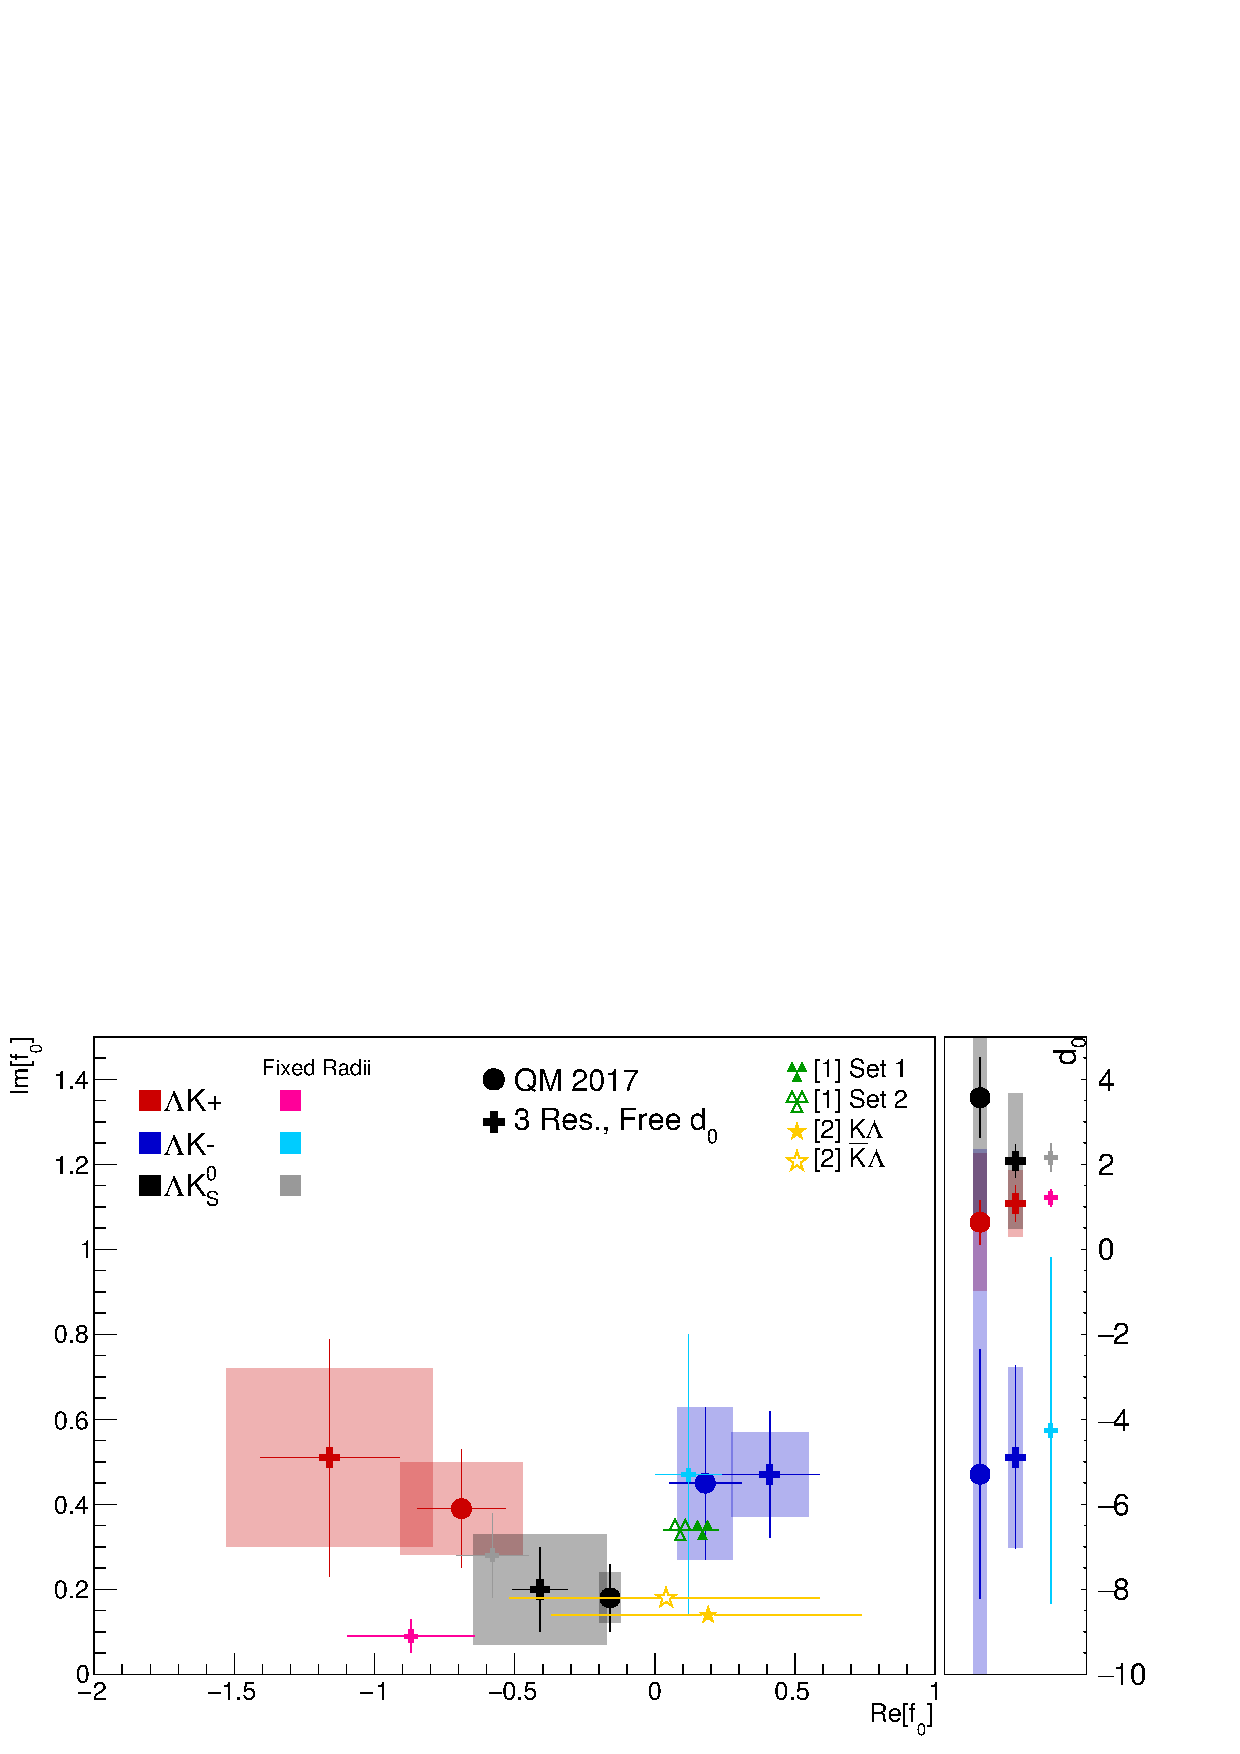
\includegraphics[width=1.0\textwidth]{/home/jesse/Analysis/FemtoAnalysis/LamKPublication/Figures/20171227/PDF/CompareAllReF0vsImF0AcrossAnalyses_3Res_10and3SeparateOnly_FreeD0Only_wFixedRadiiResults_wScattLenPredictions.pdf}% Here is how to import EPS art
\caption{\label{fig:epsart} A figure caption. The figure captions are
automatically numbered.}
\end{figure}

\begin{figure}[b]
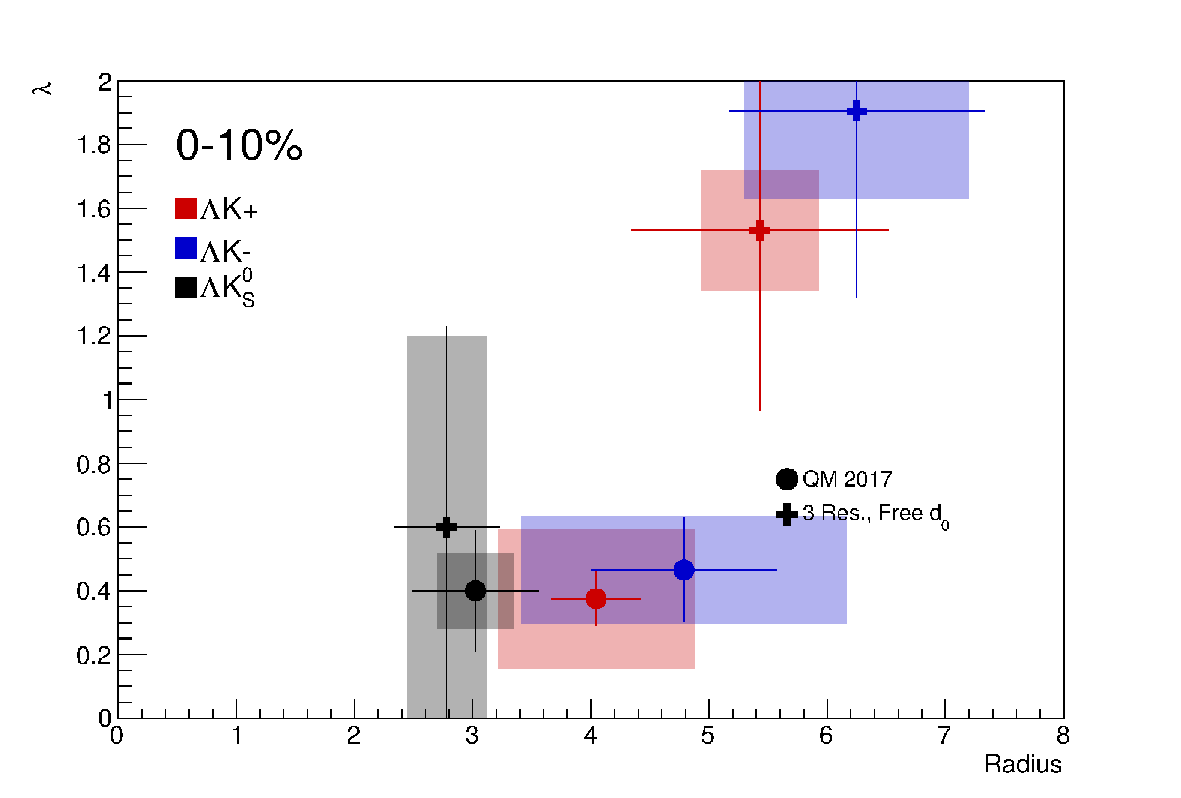
\includegraphics[width=1.0\textwidth]{/home/jesse/Analysis/FemtoAnalysis/LamKPublication/Figures/20171227/PDF/CompareAllRadiusvsLambdaAcrossAnalyses_0010_3Res_10and3SeparateOnly_FreeD0Only.pdf}% Here is how to import EPS art
\caption{\label{fig:epsart} A figure caption. The figure captions are
automatically numbered.}
\end{figure}

\begin{figure}[b]
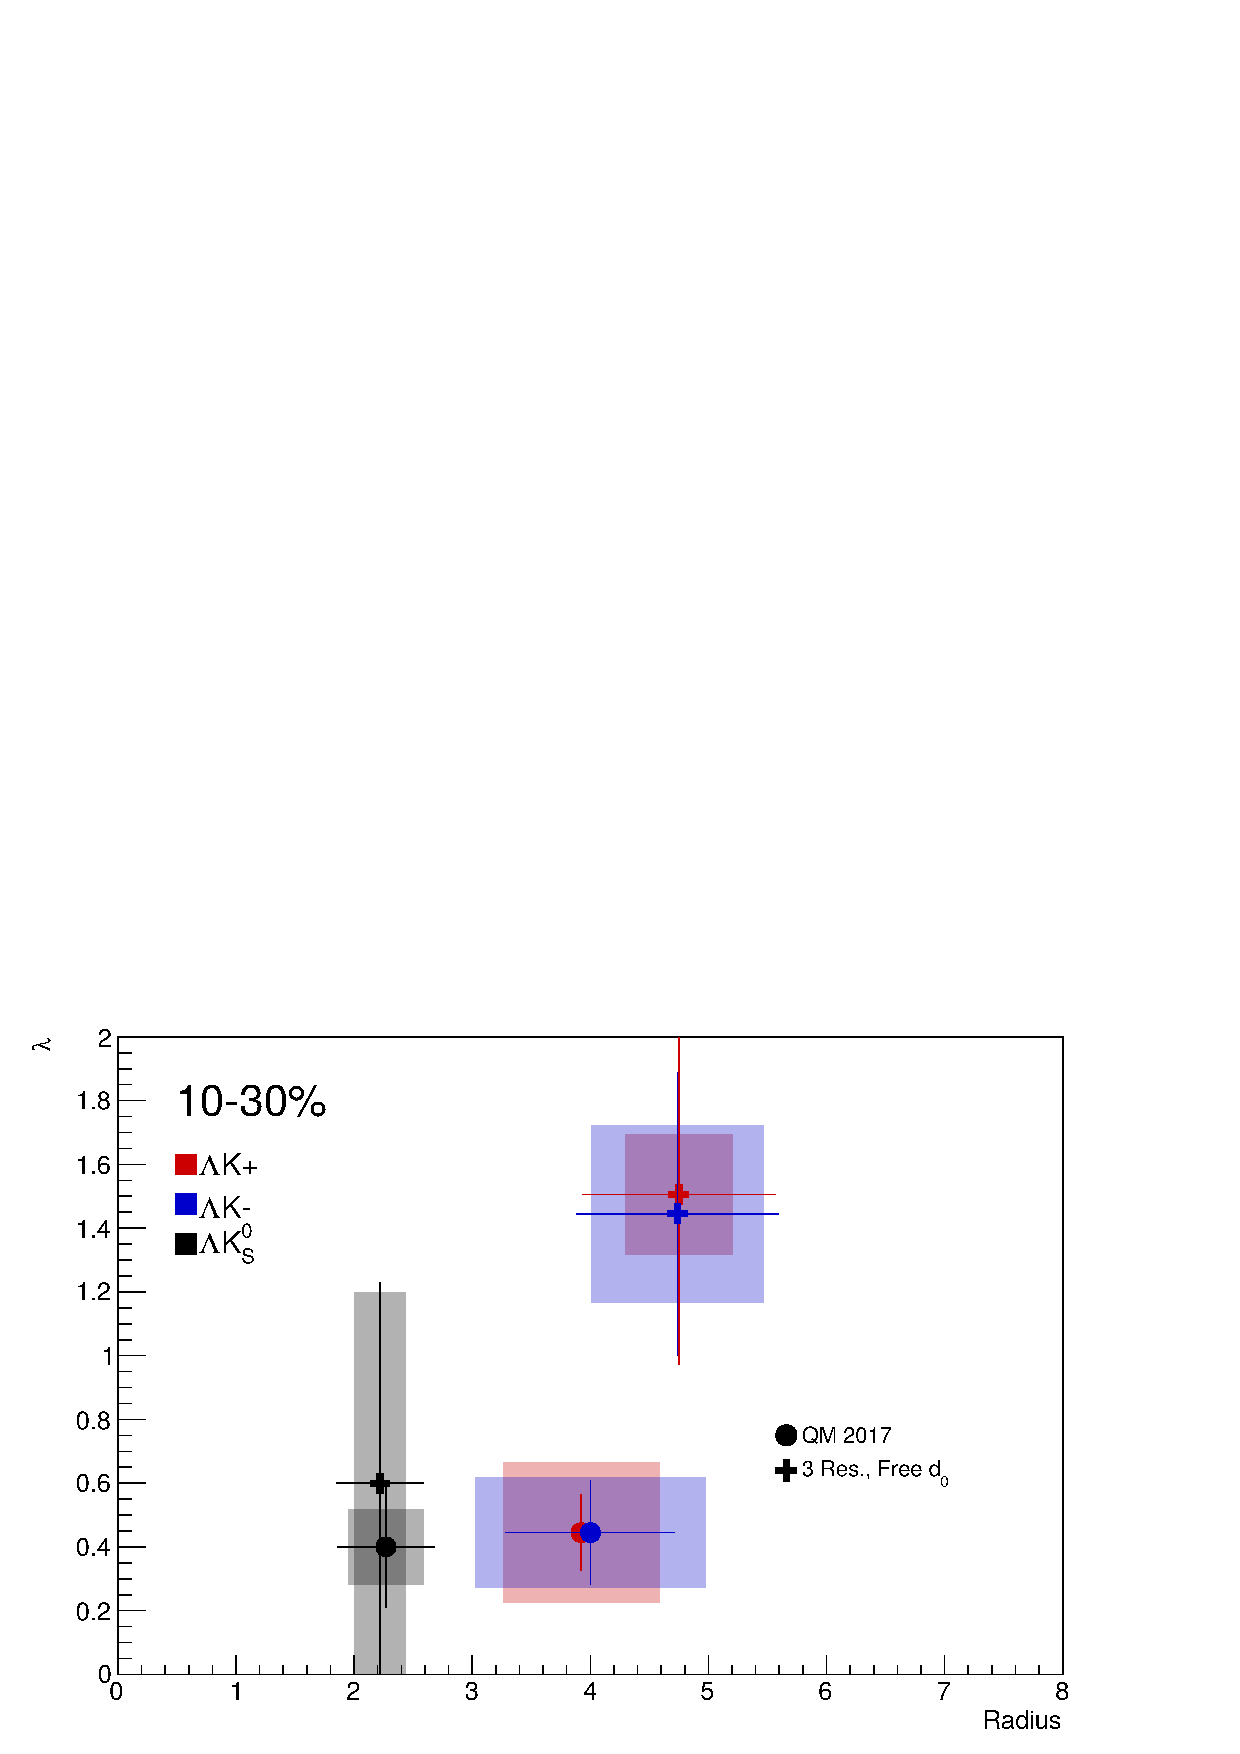
\includegraphics[width=1.0\textwidth]{/home/jesse/Analysis/FemtoAnalysis/LamKPublication/Figures/20171227/PDF/CompareAllRadiusvsLambdaAcrossAnalyses_1030_3Res_10and3SeparateOnly_FreeD0Only.pdf}% Here is how to import EPS art
\caption{\label{fig:epsart} A figure caption. The figure captions are
automatically numbered.}
\end{figure}

\begin{figure}[b]
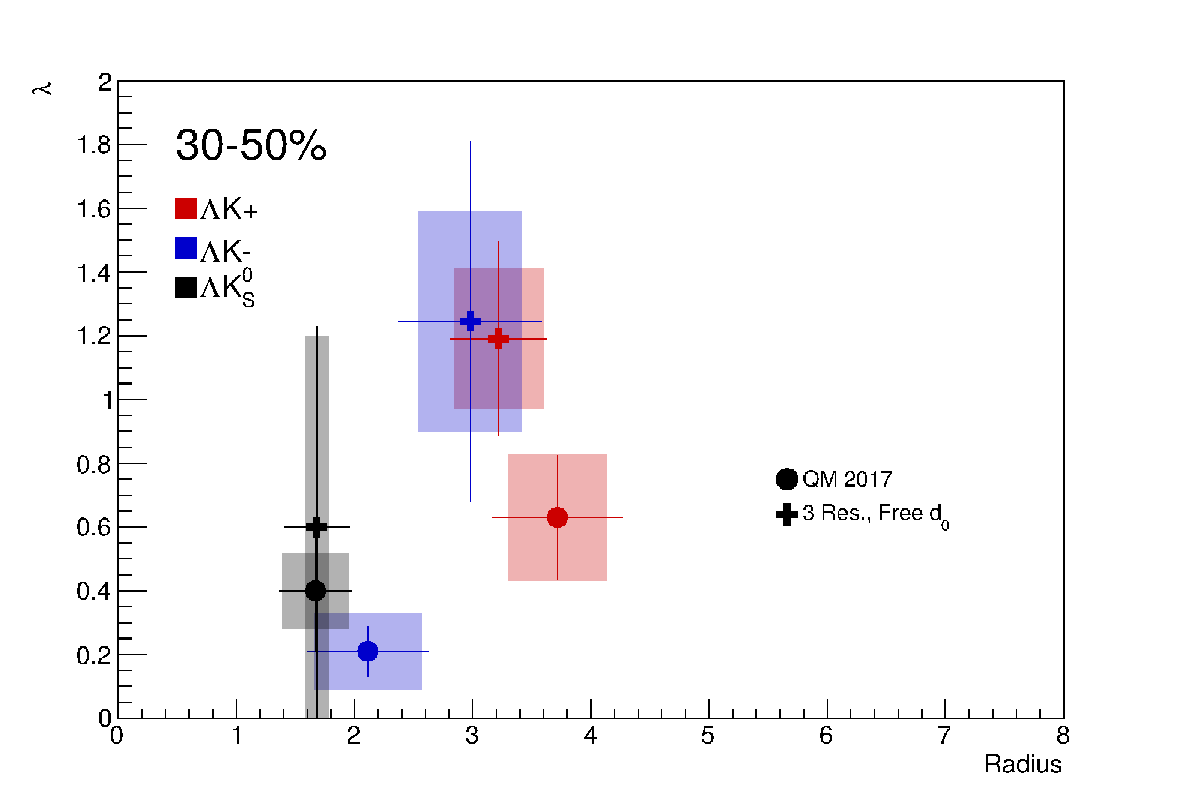
\includegraphics[width=1.0\textwidth]{/home/jesse/Analysis/FemtoAnalysis/LamKPublication/Figures/20171227/PDF/CompareAllRadiusvsLambdaAcrossAnalyses_3050_3Res_10and3SeparateOnly_FreeD0Only.pdf}% Here is how to import EPS art
\caption{\label{fig:epsart} A figure caption. The figure captions are
automatically numbered.}
\end{figure}

\begin{figure}[b]
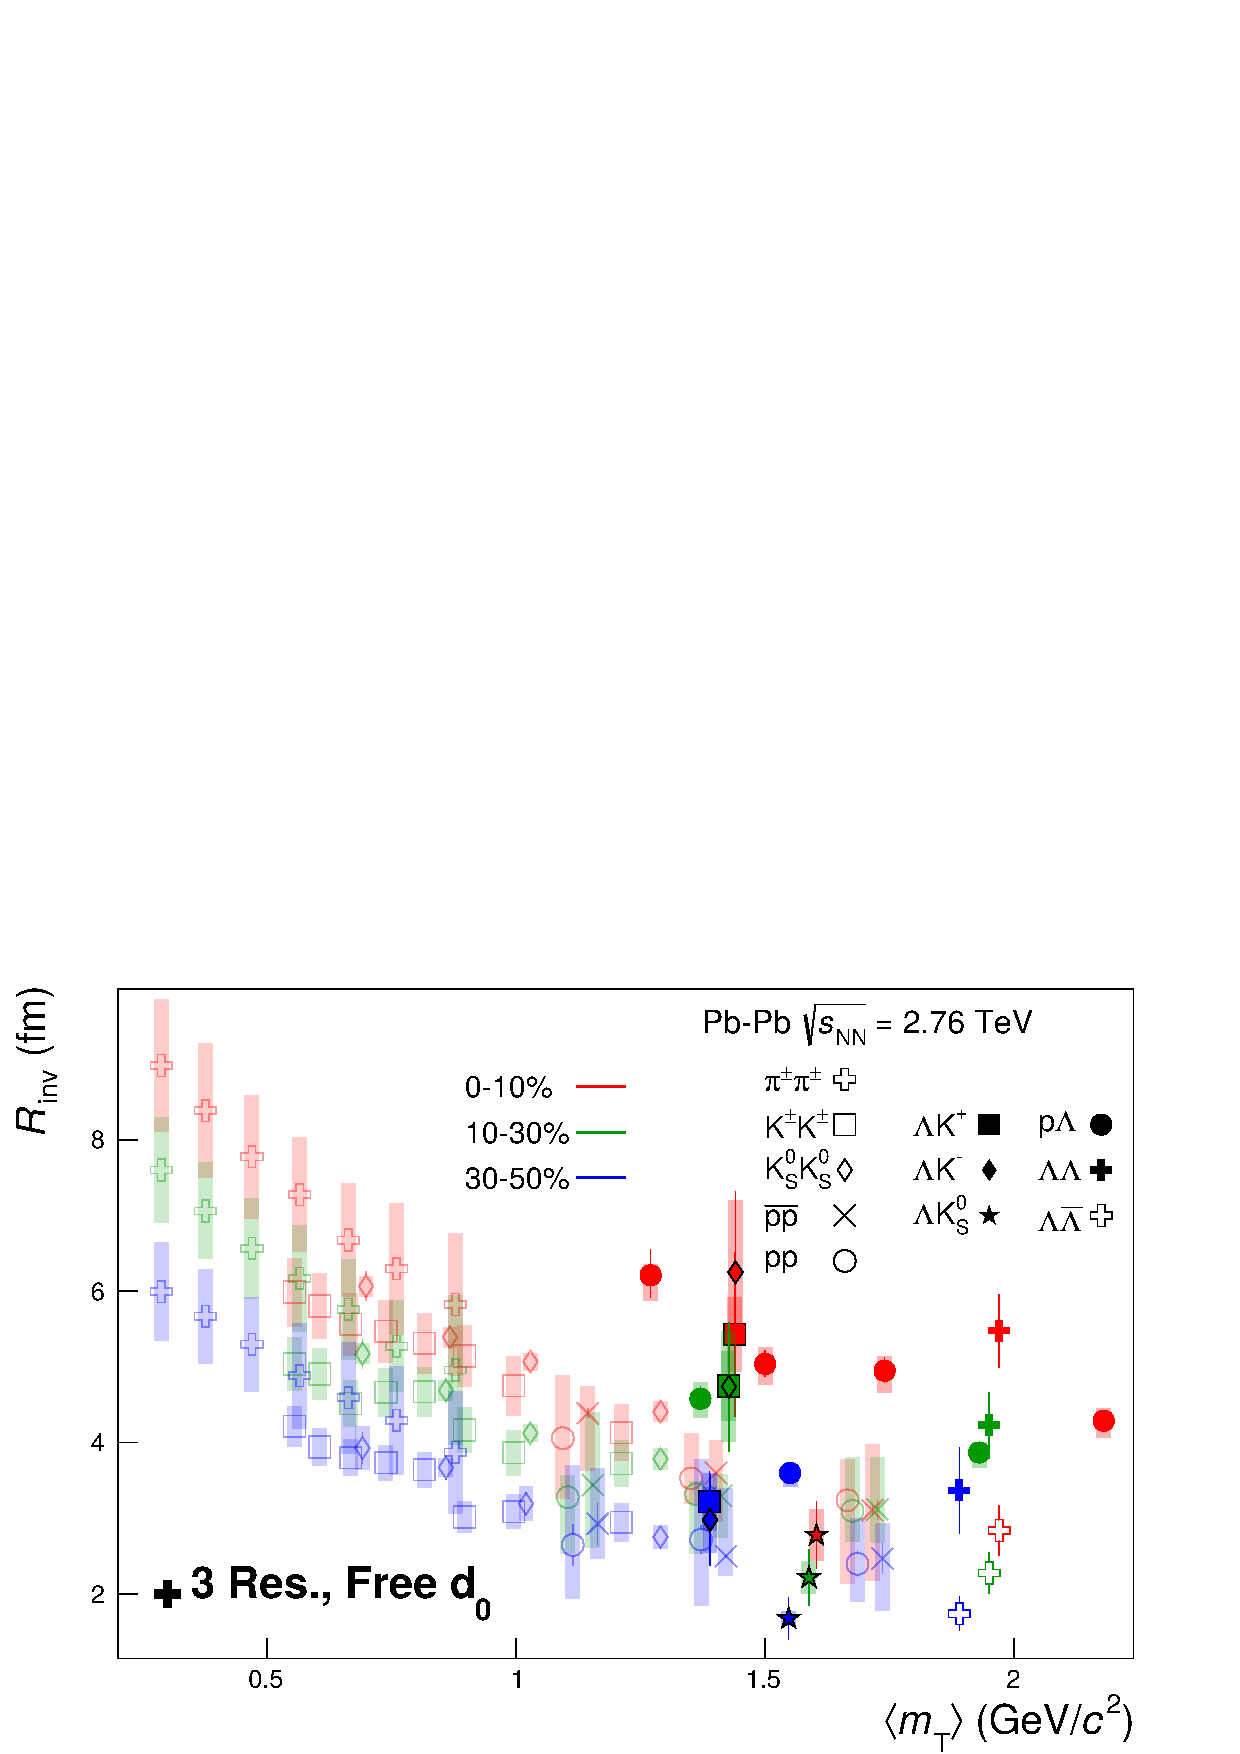
\includegraphics[width=1.0\textwidth]{/home/jesse/Analysis/FemtoAnalysis/LamKPublication/Figures/20171227/PDF/mTscaling_MinvCalc_OutlinedPoints_OthersTransparent_3Res_FreeD0.pdf}% Here is how to import EPS art
\caption{\label{fig:epsart} A figure caption. The figure captions are
automatically numbered.}
\end{figure}

\begin{figure}[b]
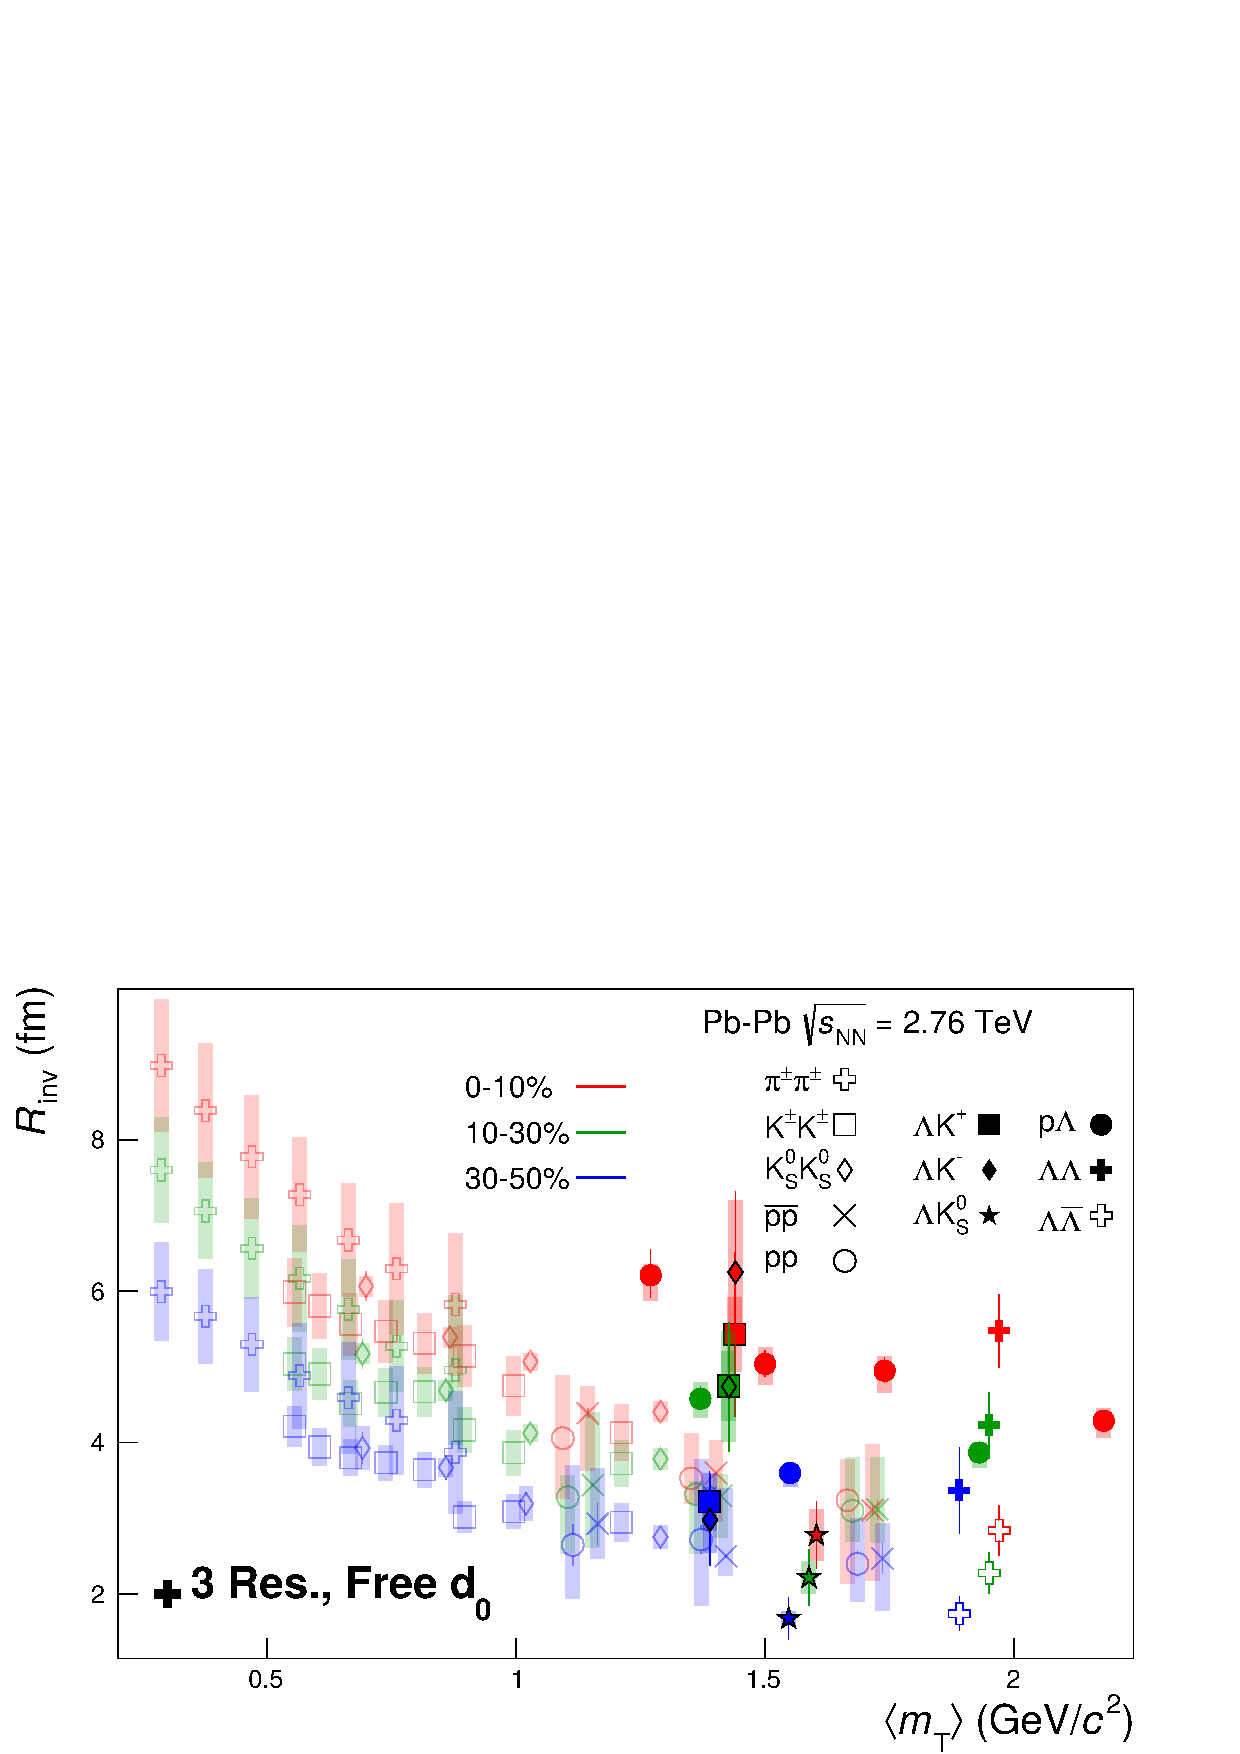
\includegraphics[width=1.0\textwidth]{/home/jesse/Analysis/FemtoAnalysis/LamKPublication/Figures/20171227/PDF/mTscaling_MinvCalc_OutlinedPoints_OthersTransparent_3Res_FreeD0.pdf}% Here is how to import EPS art
\caption{\label{fig:epsart} A figure caption. The figure captions are
automatically numbered.}
\end{figure}

\section{Summary}
\label{sec:Summary}
We did physics, and we found physics.

%%%%% acknowledgements
\newenvironment{acknowledgement}{\relax}{\relax}
\begin{acknowledgement}
\section*{Acknowledgements}
%\input{acknowledgements.tex}    %%%%%%% done by webmaster team
\end{acknowledgement}

%%%%%%%% Bibliography (In case of using bibtex generate the bbl requested by arXiv)
%\bibliographystyle{utphys}   % Remember we use title in the biblio
%\bibliography{biblio}
%\input {bibliography.tex}  

%%%%%%%%% appendix with author list
\newpage
\appendix
%
%\input{}               %%%%%%%%%%% put your appendices here
%
\section{The ALICE Collaboration}
\label{app:collab}
%\input{authorlist-preprint.tex}  %%%%%%% done by webmaster team
\end{document}
